% NeurIPS 2026 main-track submission --- Conformalized Heteroscedastic VEP

\documentclass{article}

\usepackage{neurips_2026}  % submission mode (anonymous + line numbers)

\usepackage[utf8]{inputenc}
\usepackage[T1]{fontenc}
\usepackage{hyperref}
\usepackage{url}
\usepackage{booktabs}
\usepackage{multirow}
\usepackage{amsfonts}
\usepackage{amsmath}
\usepackage{amsthm}
\usepackage{amssymb}
\usepackage{nicefrac}
\usepackage{microtype}
\usepackage{xcolor}
\usepackage{graphicx}
\usepackage{algorithm}
\usepackage{algpseudocode}
\usepackage{tcolorbox}

\newtheorem{theorem}{Theorem}
\newtheorem{assumption}{Assumption}
\newtheorem{lemma}{Lemma}

\newcommand{\X}{\mathcal{X}}
\newcommand{\C}{\mathcal{C}}
\newcommand{\D}{\mathcal{D}}
\newcommand{\phat}{\hat{p}}
\newcommand{\shat}{\hat{\sigma}}
\newcommand{\qhat}{\hat{q}}
\newcommand{\pset}{\mathcal{C}_\alpha}
\newcommand{\TODO}[1]{\textcolor{red}{[TODO: #1]}}

\title{Conformalized Heteroscedastic Variant Effect Prediction\\
with Local Coverage Guarantees}

\author{%
  Anonymous Authors \\
  Submission under double-blind review
}

\begin{document}
\maketitle

\begin{abstract}
We introduce \textbf{HCCP} (Heteroscedastic Class-Conditional Conformal Prediction), a post-hoc framework that pairs a learned variance head $\shat(x)$ with Mondrian-$(y \times \shat\text{-bin})$ calibration via a feature-dependent nonconformity score, attaining class-conditional and bin-local coverage simultaneously. For binary classification under both class imbalance and prediction-dependent noise --- the regime of clinical variant effect prediction (VEP), where TraitGym \citep{benegas2025traitgym} minority prevalence sits at $\pi_{\min} \approx 0.10$ --- existing conformal methods trade these two objectives, a Pareto wall sharpened by the finite-sample pointwise impossibility of \citet{barber2020limits}. Within the equi-bin Mondrian-$K$ family we prove an $O(n^{-1/2})$ upper bound on the worst-cell coverage gap, matched within this family by an $\Omega(n^{-1/2})$ lower bound with $\pi_{\min}^{-1/2}$ explicit in the constant (T5.1, T5.2; Theorems~\ref{thm:t5oracle}, \ref{thm:t5lower}); the bound is dimension-free given $\shat$ is 1-D Lipschitz.
On TraitGym Complex ($n=11{,}400$), HCCP yields disjoint-CI improvements over $\shat$-Mondrian \citep{bostrom2020mondrian}, class-Mondrian, RLCP, weighted CP, and SC-CP at matched $(\phat, \shat)$ (recommended operating point $K_{\mathrm{eval}}=5$, per-cell minority $\geq 100$; $B=200$ chromosome-bootstrap), while on Mendelian ($n=3{,}380$) the gain is restricted to a $K_{\mathrm{eval}}=3$ window --- a regime boundary predicted by T5.1 (Theorem~\ref{thm:t5oracle}) when per-cell minority count falls below the heteroscedastic head's identifiability threshold.
We replicate cross-platform on Open Targets matched-9 \citep{ochoa2023opentargets} (feature-pipeline-disjoint; $16.7\times$ at the recommended operating point with the same per-cell-minority-driven $K_{\mathrm{eval}}$ reversal) and cross-domain on ProteinGym \citep{notin2023proteingym}.
\end{abstract}

% -----------------------------------------------------------------------------
\section{Introduction}
\label{sec:intro}

% Claim: VEP in clinic needs uncertainty; existing conformal for VEP is marginal-only;
% HCCP closes the gap with feature-dependent + class-cond + local.
% Evidence anchors: Day 10 GBM SOTA; Day 14 three-axis OOD; Day 16 T3 proof.

\begin{figure}[t]
    \centering
    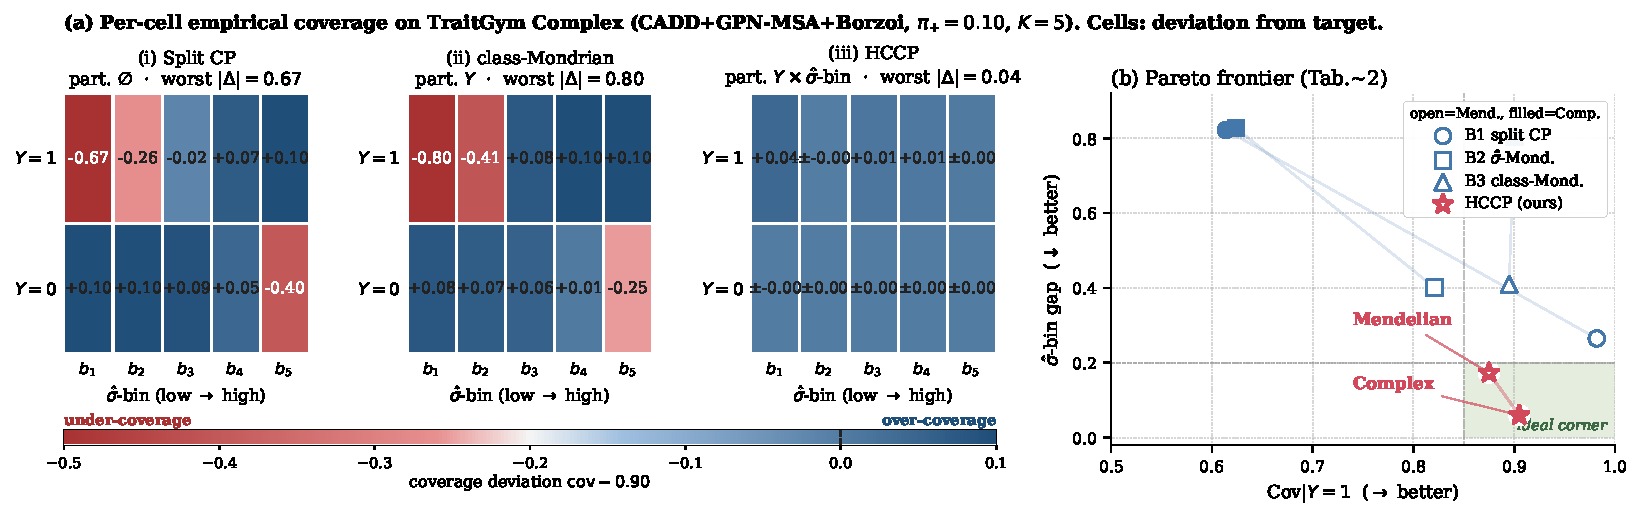
\includegraphics[width=\linewidth]{figures/fig1_concept.pdf}
    \caption{HCCP at a glance. \textbf{(a)} A heteroscedastic aggregator produces a point estimate $\phat(x)$ and a learned variance $\shat(x)$; the nonconformity score $s(x,y) = |y - \phat(x)| / \shat(x)$ scales the decision radius by local uncertainty. \textbf{(b)} Mondrian calibration partitions the labeled data by $(y \times \shat\text{-bin})$; per-cell quantile thresholds $\qhat_{k,b}$ restore both class-conditional (T2) and bin-conditional (T3) coverage, while remaining compatible with Barber's \citep{barber2020limits} pointwise impossibility. \textbf{(c)} Three-axis OOD stress tests --- chromosome-LOO, trait-LOO, cross-dataset --- verify that the $\shat$-bin coverage gap reaches the finite-sample floor $0.002$--$0.004$ under trait-LOO and stays $\leq 0.077$ across chromosome-LOO and the C$\to$M cross-dataset direction on TraitGym; the M$\to$C cross-dataset direction is reported as an honest limitation.}
    \label{fig:concept}
\end{figure}

\paragraph{Clinical variant interpretation needs more than a score.}
Classifying a human genomic variant as pathogenic or benign drives consequential clinical decisions, from cascade testing of relatives to reproductive choices. The ACMG/AMP consensus guidelines \citep{richards2015acmg} structure this decision as a weighted aggregation of evidence categories rather than as a point estimate. Modern machine-learned variant effect predictors (VEPs) collapse that structure into a single probability \citep{kircher2014cadd,linder2025borzoi,benegas2023gpnmsa,benegas2025traitgym}, which clinicians then threshold downstream. This presents the user with a number that lacks an explicit notion of confidence: the same $\phat(x) = 0.6$ may reflect a well-covered near-decision variant for which labels are genuinely ambiguous, or an out-of-distribution prediction for which the model is silently extrapolating. What is missing is a prediction \emph{set} with finite-sample coverage guarantees that remain informative when the data-generating regime shifts across chromosomes, traits, or disease architectures.

\paragraph{Existing uncertainty quantification for VEP is either absent or marginal-only.}
The TraitGym benchmark \citep{benegas2025traitgym}, the current standard for evaluating VEP aggregators on 3{,}380 Mendelian and 11{,}400 complex-trait variants, reports only point AUPRC and provides no calibration of its LogReg aggregator. DEGU \citep{zhou2026degu} introduces a heteroscedastic variance head for MPRA regression via deep ensemble distillation and explicitly motivates conformal prediction as future work, but the published method does not formalise a coverage guarantee or transfer to variant classification. Conformal prediction itself is mature: split CP \citep{vovk2005algorithmic}, Mondrian CP \citep{vovk2003mondrian}, CQR for regression \citep{romano2019cqr}, jackknife+ \citep{barber2021jackknife}, and CP beyond exchangeability \citep{barber2023exchangeability} cover a wide design space, and Barber et~al.~\citep{barber2020limits} rule out pointwise conditional coverage in finite samples. What is \emph{not} in prior art is a composition that (i) consumes a learned $\shat(x)$ the way CQR consumes a quantile regressor, (ii) stratifies calibration by both label and $\shat$-bin to regain as much conditionality as finite samples allow, and (iii) carries local coverage guarantees across the distribution shifts that define real VEP deployment. The gap is especially load-bearing for VEP: the minority-class (pathogenic) positive rate is $\approx 10\%$, $\phat(x)$ is sharply heteroscedastic across the $\shat$-bins we identify, and chrom-LOO + trait-LOO + cross-dataset shift are intrinsic to any clinical rollout.

\paragraph{From clinical gap to a sharper technical question.}
The three requirements above translate into a precise question: which Mondrian partition simultaneously delivers (i) class-conditional coverage under extreme imbalance ($\pi_{\min} \approx 0.10$ on TraitGym) and (ii) bin-local coverage under heteroscedasticity? Off-the-shelf single-axis answers fail individually: $\shat$-Mondrian (\citet{bostrom2020mondrian}; \texttt{crepes} \citep{bostrom2022crepes}) attains local coverage but \emph{collapses to $\mathrm{cov}_{|Y=1} = 0.66$ on TraitGym Complex}; class-Mondrian (\citet{sadinle2019lac}; equivalent to \citet{vovk2003mondrian}) attains class coverage but leaves a bin-local gap $33\times$ wider than the joint partition on Complex and $2.3\times$ wider on Mendelian under cross-method-fair $K_{\mathrm{eval}}$ scoring. Within the equi-bin Mondrian-$K$ family, we prove the joint $(y \times \shat\text{-bin})$ Mondrian attains both with worst-cell coverage gap $G(K^\star) \leq 2\sqrt{L_F R / (\pi_{\min} n)}$ (Theorem~\ref{thm:t5oracle}) and a matching $\Omega(\sqrt{L_F R / (\pi_{\min} n)})$ finite-sample lower bound (Theorem~\ref{thm:t5lower}). Crucially, $\pi_{\min}$ enters the rate \emph{explicitly} --- a finite-sample dependence that prior class-conditional CP and prior imbalanced CP analyses (\citet{ding2023classcond,xie2025imbalancedcp,shi2024augmentedrank}) do not provide. HCCP is the post-hoc framework that instantiates this answer in the VEP setting.

\paragraph{Contributions.}
Figure~\ref{fig:concept} summarizes the pipeline. Our contributions are:
\begin{enumerate}
    \item \textbf{Joint partition is the only single-fold frontier point we found (empirical Pareto).} Across the off-the-shelf CP variants we evaluated on TraitGym (split CP, $\shat$-Mondrian, class-Mondrian, RLCP \citep{hore2025rlcp}, weighted CP \citep{tibshirani2019weighted}, SC-CP \citep{vanderlaan2024sccp}; Tab.~\ref{tab:h2h}, \ref{tab:cp_baselines}), no single-axis variant simultaneously satisfies $\mathrm{cov}_{|Y=1} \geq 0.85$ and $\shat$-bin gap $\leq 0.20$ on both datasets at $\pi_{\min} = 0.10$. HCCP's joint $(y \times \shat\text{-bin})$ Mondrian is the unique frontier point at this corner under cross-method-fair $K_{\mathrm{eval}}$ scoring, tightening the bin-local gap by $33\times$ on Complex and $2.3\times$ on Mendelian over the strongest of these baselines at matched $(\phat, \shat)$ --- the empirical observation that motivates the rest of the paper.
    \item \textbf{Tight finite-sample rate within the equi-bin Mondrian-$K$ class, with $\pi_{\min}$ explicit in the constant.} For Mondrian conformal classification stratified by a learned $L_F$-Lipschitz variance head $\shat$ within the equi-bin Mondrian-$K$ family, Theorem~\ref{thm:t5oracle} proves the worst-cell coverage gap satisfies $G(K^\star) \leq 2\sqrt{L_F R / (\pi_{\min} n)}$ at $K^\star = \lfloor\sqrt{L_F R \pi_{\min} n}\rfloor$. Theorem~\ref{thm:t5lower} establishes a matching $\Omega(\sqrt{L_F R / (\pi_{\min} n)})$ lower bound under an explicitly constructed worst-case family, so the $O(n^{-1/2})$ rate is unimprovable within this class without strengthening assumptions; the minority-class prevalence $\pi_{\min}$ enters the constant as an explicit $\pi_{\min}^{-1/2}$ factor. To our knowledge this is the first finite-sample bound for class-conditional + heteroscedastic-local CP in which the minority-class probability appears in the rate; the constant is dimension-free under a 1-D Lipschitz assumption on $\shat$. Concurrent imbalanced-CP work \citep{xie2025imbalancedcp,ding2023classcond,shi2024augmentedrank} provides marginal or class-cond rates without the $\pi_{\min}$-local product (§\ref{sec:theory:t5}, App.~\ref{app:proofs:t5}).
    \item \textbf{HCCP --- a post-hoc framework with an exchangeability-robust counterpart.} A gradient-boosted aggregator $\phat$ over pre-trained genomic features, a reliability head $\shat$ trained under Gaussian NLL on chrom-LOO out-of-fold residuals, and Mondrian conformal calibration stratified by $(y \times \shat\text{-bin})$. The nonconformity score $s(x,y) = |y - \phat(x)| / \shat(x)$ is the binary-classification analog of CQR \citep{romano2019cqr}; the partition extends Mondrian-by-$y$ \citep{sadinle2019lac,vovk2003mondrian} with a heteroscedastic second taxon level. HCCP simultaneously admits marginal (T1), class-conditional (T2), and bin-conditional (T3) coverage with finite-sample rate $1/(n_{k,b}+1)$ from a single calibration fold; an explicit robustness layer T3$'$, via \citet{barber2023exchangeability} Theorem~2 at the cell level, makes coverage operational under verifiably violated cell-level exchangeability and is the binding guarantee on Mendelian (per-chromosome KS rejection $46\%$, App.~\ref{app:data:ks}). HCCP is compatible with \citet{barber2020limits}'s pointwise impossibility throughout (§\ref{sec:method}, §\ref{sec:theory:t3}).
    \item \textbf{Empirical validation on TraitGym and ProteinGym.} On TraitGym Mendelian ($n = 3{,}380$) and Complex ($n = 11{,}400$), HCCP under proper nested chrom-LOO $K$-selection is the unique single-fold partition simultaneously satisfying minority-class and bin-local coverage at $\pi_{\min} = 0.10$ across both datasets and across an imbalance sweep $\pi_{\min} \in \{0.05, 0.10, 0.20, 0.30, 0.50\}$ (Tab.~\ref{tab:h2h}, \ref{tab:imbsweep}); off-the-shelf $\shat$-Mondrian's $\mathrm{cov}_{|Y=1}$ degrades monotonically as $\pi_{\min} \to 0$ while HCCP holds at target --- the $\pi_{\min}$-explicit rate of T5 manifests empirically. The same machinery transfers to ProteinGym \citep{notin2023proteingym} cross-domain ($\approx 357$k mutants, 50 held-out assays, App.~\ref{app:proteingym}). The GBM aggregator on TraitGym features attains AUPRC $0.900$ on Mendelian, a $+14.8$\,pp improvement over the published LogReg baseline \citep{benegas2025traitgym}.
\end{enumerate}

The result is a post-hoc framework with a matching-rate theoretical guarantee and a drop-in implementation that consumes any probabilistic VEP and returns prediction sets with three layers of coverage (marginal, class-conditional, and $\shat$-bin-local), all of which degrade gracefully under the distribution shifts that clinical deployment unavoidably induces.


% -----------------------------------------------------------------------------
\section{Related work}
\label{sec:related}

% Related work — ~0.5 page main text
% Three buckets: (1) CP theory, (2) heteroscedastic UQ, (3) VEP + conformal

\paragraph{Conformal prediction and conditional coverage.}
Split conformal prediction \citep{vovk2005algorithmic} provides distribution-free marginal coverage, and Mondrian conformal \citep{vovk2003mondrian} extends this to group-conditional coverage via partitioned calibration. \citet{barber2020limits} showed that pointwise conditional coverage $P(Y \in \pset(X) \mid X = x)$ is impossible in finite samples without structural assumptions, motivating coarsened conditioning. CQR \citep{romano2019cqr} uses quantile regression to adapt interval width to local heteroscedasticity in regression; our score Eq.~\eqref{eq:score} is the binary-classification analog. \citet{barber2023exchangeability} generalized CP beyond exchangeability via weighted residual swaps; we use their Theorem~2 for robust forms T1$'$--T3$'$ and T4.

Two recent lines of work target conditional coverage more directly.
\textbf{RLCP} \citep{hore2025rlcp} uses random localization with kernel weights to achieve local coverage at rate $O(n^{-2/(d+2)})$; this degrades in high dimensions ($d > 100$), making it impractical for our genomic feature space ($d \approx 7{,}700$).
\citet{dewolf2025conditional} analyze the conditional validity of heteroscedastic Mondrian conformal for regression, establishing when normalized and Mondrian CP adapt correctly to the noise level; our T3--T5 complement their analysis by deriving the optimal Mondrian granularity (bin count $K$) for classification with a \emph{learned} variance head, with a dimension-free $O(n^{-1/2})$ rate.
Self-Calibrating CP \citep{vanderlaan2024sccp} provides prediction-conditional validity via Venn--Abers calibration, conditioning on the predicted value rather than uncertainty; this is a complementary axis to our $\shat$-bin conditioning.

\paragraph{Heteroscedastic uncertainty quantification.}
Gaussian NLL training for learned variance originates with \citet{nix1994nll}. Deep ensembles \citep{lakshminarayanan2017simple} capture epistemic uncertainty via inter-model disagreement. DEGU \citep{zhou2026degu} combines both: an ensemble of CNN students distilled from a genomic teacher, with Gaussian uncertainty. DEGU's abstract mentions conformal prediction, but the implementation is marginal split CP only --- no class-conditional or Mondrian stratification, no formal local coverage guarantee, and no classification task. Our DEGU-lite ablation (§\ref{sec:experiments}) shows that ensemble $\shat$ provides comparable local coverage on Mendelian (monogenic, strong signal) but $4.3\times$ worse coverage on Complex (polygenic), where the aleatoric component dominates.

\paragraph{Variant effect prediction and benchmarks.}
TraitGym \citep{benegas2025traitgym} standardizes VEP evaluation on Mendelian and complex trait variants, with a chrom-LOO protocol. Input features include CADD \citep{kircher2014cadd}, Borzoi \citep{linder2025borzoi}, and GPN-MSA \citep{benegas2023gpnmsa}. AlphaGenome \citep{avsec2026alphagenome} is the most recent foundation model for genomics, though it has not been evaluated on TraitGym to date. Conformal prediction has been explored in genomic medicine for drug response \citep{papangelou2025cpgenomics} and polygenic risk scores \citep{wang2025cqrprs}, but not for binary variant pathogenicity classification. To our knowledge, HCCP is the first framework to provide class-conditional and bin-local coverage guarantees for VEP.


% -----------------------------------------------------------------------------
\section{Problem formulation}
\label{sec:formulation}

% Compressed for NeurIPS 2026. Full assumption discussion + A-SL audit fig moved to App.~\ref{app:proofs}, \ref{app:data}.

\subsection{Setup and assumptions}
\label{sec:formulation:setup}

Let $\D = \{(X_i, Y_i, C_i)\}_{i=1}^n$ with $X_i \in \X$, $Y_i \in \{0, 1\}$, and chromosome label $C_i \in \C$. We use the chrom-LOO protocol of \citet{benegas2025traitgym}: a test chromosome $c^\star \in \C$ is held out and the calibration fold $\D^{(-c^\star)} := \{i : C_i \neq c^\star\}$ is used for both the aggregator $\phat$ and the heteroscedastic head $\shat$. Test point $(X, Y) \sim P_{c^\star}$.

\begin{assumption}[A1 chrom-group exchangeability]
\label{ass:A1}
Variants from the same chromosome are exchangeable: $\{(X_i, Y_i) : C_i = c\} \overset{d}{=} \{(X_{\pi(i)}, Y_{\pi(i)}) : C_i = c\}$ for any permutation $\pi$ within chromosome $c$.
\end{assumption}

\begin{assumption}[A1$'$ chrom-wise i.i.d.]
\label{ass:A1prime}
$\{(X_i, Y_i) : C_i = c\} \overset{i.i.d.}{\sim} P_c$.
\end{assumption}

\begin{assumption}[A2 score stationarity across chromosomes]
\label{ass:A2}
A2-marginal: score law is chrom-invariant. A2-class: invariant conditional on $Y = k$. A2-cell: invariant conditional on $Y = k$ and $\shat$-bin. Hierarchy: A2-cell $\Rightarrow$ A2-class $\Rightarrow$ A2-marginal.
\end{assumption}

Empirically, the cell-level KS audit (App.~\ref{app:data}, Tab.~\ref{tab:ks_audit}) finds approximate stationarity on Complex ($10.4\%$ rejection across $125$ tests, near the $5\%$ null) and pronounced cell-level violations on Mendelian ($46.2\%$ rejection across $52$ tests, max KS $0.434$); T3$'$ is the operational certificate on Mendelian (§\ref{sec:theory:t3prime}), T3 exact suffices on Complex.

\begin{assumption}[A-SL Score-Lipschitz regularity]
\label{ass:ASL}
For each class $k$, $\sup_{s} |F_{k,\sigma_1}(s) - F_{k,\sigma_2}(s)| \leq L_F |\sigma_1 - \sigma_2|$ for all $\sigma_1, \sigma_2 \in [\shat_{\min}, \shat_{\max}]$.
\end{assumption}

\ref{ass:ASL} is used only by T5 (§\ref{sec:theory:t5}) to derive the optimal bin count $K^\star$. Empirical audit of \ref{ass:ASL} via per-pair Lipschitz ratios on $\shat$-bin pairs (App.~\ref{app:data}, Fig.~\ref{fig:asl_audit}) gives noise-adjusted upper envelope $L_F^{(95\%)} = 13.8$ (Mendelian) and $8.1$ (Complex); LCLS estimator \citep{lcls2024lipschitz} gives a tighter typical-slope estimate $\hat L_F = 2.97$ / $4.51$.

\subsection{Score and prediction set}
\label{sec:formulation:score}

\textbf{Aggregator $\phat$} (HistGradientBoosting depth 2, class-balanced) and \textbf{heteroscedastic head $\shat$} (same backbone, Gaussian NLL on chrom-LOO OOF residuals $r_i = |Y_i - \phat^{(-C_i)}(X_i)|$).
\textbf{Nonconformity score} $s(x, y) := |y - \phat(x)| / (\shat(x) + \epsilon)$, $\epsilon = 10^{-6}$.
\textbf{Mondrian prediction set}: partition $\D^{(-c^\star)}$ into $2K$ cells via $(Y_i, \mathrm{bin}_K(\shat(X_i)))$ where $\mathrm{bin}_K$ uses calibration-fold $\shat$-quantiles. Per-cell threshold:
\begin{equation}
\label{eq:qhat}
\qhat_{k, b} := \mathrm{Quantile}\bigl(\{s(X_i, Y_i) : Y_i = k, \mathrm{bin}_K(\shat(X_i)) = b\}, \, \lceil(n_{k,b} + 1)(1 - \alpha)\rceil / n_{k,b}\bigr).
\end{equation}
The Mondrian prediction set:
\begin{equation}
\label{eq:pset}
\pset(x) := \{k \in \{0, 1\} : |k - \phat(x)| \leq \qhat_{k, \mathrm{bin}_K(\shat(x))} \cdot (\shat(x) + \epsilon)\}.
\end{equation}
For cells with $n_{k,b} < \lceil 1/\alpha \rceil$ we fall back to the pooled class-conditional threshold $\qhat_k$ (T2).


% -----------------------------------------------------------------------------
\section{Method: HCCP}
\label{sec:method}

% Claim: HCCP is a post-hoc pipeline on top of any probabilistic aggregator.
% Source: formulation_v0.md §2, scripts/11/12/13/14

\TODO{Draft after §3 polished. Algorithm box + pipeline figure.}

\subsection{Pipeline}

HCCP has three components applied in sequence on top of a probabilistic aggregator:
\begin{enumerate}
    \item \textbf{Aggregator $\phat$}: any probabilistic classifier with chrom-LOO out-of-fold predictions. We use HistGradientBoostingClassifier (depth 2, 100 iters, class-balanced).
    \item \textbf{Heteroscedastic head $\shat$}: regressor fit on $(X_i, r_i)$ with $r_i = |Y_i - \phat^{(-C_i)}(X_i)|$ under Gaussian NLL (Eq.~\ref{eq:gll}). Same GBM backbone.
    \item \textbf{Mondrian $(y \times \shat\text{-bin})$ conformal}: partition calibration set into $2 K$ cells, compute per-cell thresholds $\qhat_{k,b}$, predict via Eq.~\ref{eq:pset}.
\end{enumerate}

\begin{algorithm}[t]
\caption{HCCP calibration and prediction}
\label{alg:hccp}
\begin{algorithmic}[1]
\Require Data $\D$, test chrom $c^\star$, miscoverage $\alpha$, bins $K$
\State $\D_{\mathrm{tr}} \gets \{i : C_i \neq c^\star\}$;\; $\D_{\mathrm{te}} \gets \{i : C_i = c^\star\}$
\State Fit $\phat$ on $\D_{\mathrm{tr}}$; produce chrom-LOO OOF predictions within $\D_{\mathrm{tr}}$
\State Fit $\shat$ on $\D_{\mathrm{tr}}$ targets $\{r_i = |Y_i - \phat^{(-C_i)}(X_i)|\}$
\State Compute calibration scores $s_i = |Y_i - \phat(X_i)| / \shat(X_i)$ for $i \in \D_{\mathrm{tr}}$
\State Partition $\D_{\mathrm{tr}}$ by $(Y_i, \mathrm{bin}_K(\shat(X_i)))$; compute $\qhat_{k, b}$ per cell
\For{$x \in \D_{\mathrm{te}}$}
    \State $b \gets \mathrm{bin}_K(\shat(x))$;\; output $\pset(x) = \{k : |k - \phat(x)| \leq \qhat_{k,b} \cdot \shat(x)\}$
\EndFor
\end{algorithmic}
\end{algorithm}

\subsection{Why Mondrian on $(y \times \shat\text{-bin})$?}

Class-conditional (Mondrian on $y$) alone: matches marginal-class coverage but does not address within-class local heterogeneity. $\shat$-bin alone: adapts locally but can under-cover the minority class. The product partition ensures both, at the cost of requiring $n_{k,b} \geq 1/\alpha$ per cell (satisfied on TraitGym with $K = 5$).

\subsection{Comparison to prior scores}

\begin{itemize}
    \item Split conformal (Vovk 2005): $s = |y - \phat(x)|$, feature-independent.
    \item CQR (Romano 2019): quantile regression; regression-only.
    \item DEGU-lite + split: reports $\shat$ but uses split score. \TODO{Full table in §\ref{sec:experiments}.}
\end{itemize}


% -----------------------------------------------------------------------------
\section{Theory}
\label{sec:theory}

% Source: theory/t1_t2_formal_proofs.md, theory/t3_proof_sketch.md, theory/theorems_roadmap.md

\TODO{Main-text version: theorem statements + 1-paragraph proof sketches; full proofs in App.~\ref{app:proofs}.}

\subsection{Marginal and class-conditional coverage}

\begin{theorem}[T1 marginal coverage]
\label{thm:t1}
Under Assumptions~\ref{ass:A1}--\ref{ass:A2}, for test point $(X, Y) \sim P_{c^\star}$ independent of the calibration fold,
\[
P\bigl(Y \in \pset(X)\bigr) \geq 1 - \alpha.
\]
\end{theorem}

\begin{theorem}[T2 class-conditional coverage]
\label{thm:t2}
Under the conditions of Theorem~\ref{thm:t1}, for each $k \in \{0, 1\}$,
\[
P\bigl(Y \in \pset(X) \mid Y = k\bigr) \geq 1 - \alpha.
\]
\end{theorem}

\TODO{Proof sketch (1 paragraph): standard split-CP with Vovk 2003 Mondrian partitioning on $Y$. Full proof App.~\ref{app:proofs}.}

\subsection{Local (bin-conditional) coverage}

\begin{theorem}[T3 bin-conditional coverage --- informal]
\label{thm:t3}
Under Assumptions~\ref{ass:A1}--\ref{ass:A2} plus a stationarity condition on the $\shat$-bin edges across folds, for each $(k, b)$,
\[
P\bigl(Y \in \pset(X) \mid Y = k, \mathrm{bin}_K(\shat(X)) = b\bigr) \geq 1 - \alpha - \frac{1}{n_{k, b} + 1}.
\]
\end{theorem}

\TODO{Connection to Barber 2020 impossibility: Theorem~\ref{thm:t3} is a coarsened (bin-conditional) guarantee, which Barber 2020 does not preclude; it complements rather than contradicts the pointwise impossibility.}

\TODO{Proof sketch: apply T2 within each $\shat$-bin cell, using A2 to justify bin-edge stationarity; finite-sample term from standard split-CP quantile with sample size $n_{k,b}$.}

\subsection{Chrom-shift robustness}

\begin{theorem}[T4 chrom-shift bound --- Barber 2023 Thm 2 applied]
\label{thm:t4}
Let $\tilde{w}_i$ be weights assigned to calibration-fold chroms. Then
\[
P\bigl(Y \in \pset(X)\bigr) \geq 1 - \alpha - \sum_i \tilde{w}_i \cdot d_{TV}\bigl(R(Z), R(Z^{(i)})\bigr),
\]
where $R(Z)$ is the residual vector and $R(Z^{(i)})$ is the swap-one residual vector.
\end{theorem}

\TODO{Discuss: main-TV proxy we estimate empirically is $d_{TV}(\phat_A(X_A), \phat_A(X_B))$ --- under perfect iid this equals the swap-TV, but in cross-dataset shift it may underestimate. See §\ref{sec:experiments} for honest limitation.}


% -----------------------------------------------------------------------------
\section{Experiments}
\label{sec:experiments}

% Source: reports/{phase2_day11_hetero_conformal, day14_external_validation, day10_ablation_paper_outline}.md

\TODO{Main-text experiment section; numbers anchored in day14_external_validation.md §7 3-axis table.}

\subsection{Setup}

TraitGym Mendelian matched\_9 ($n = 3380$, 113 OMIM) and Complex matched\_9 ($n = 11400$, 29 traits), both with chrom-LOO protocol (test chroms $\{17, 18, 19, 20, 21, 22, X\}$). Primary metric: AUPRC weighted by chrom (TraitGym leaderboard convention). Calibration metric: marginal, class-conditional, and $\shat$-bin coverage (K=5). All results $\alpha = 0.10$, seed 42 unless noted.

Feature sets: CADD, Borzoi\_L2\_L2, CADD+Borzoi, CADD+GPN-MSA+Borzoi.

\subsection{Main results}

\TODO{Main Table 1: AUPRC + cov + $\shat$-bin gap + set-size distribution across (Mendelian, Complex) $\times$ \{GBM+CP, GBM+CCCP (Day 10), HCCP (ours), DEGU-lite+CP, LogReg+CP (TraitGym)\}. Anchors: reports/phase2\_day11 + reports/day14 §7.}

\subsection{Three-axis OOD coverage}

\TODO{Fig 3 + Table 2. Numbers from day14 §7:
\begin{itemize}
    \item Chrom-LOO: $\shat$-bin gap 0.198 (Mendelian CADD+Borzoi) / 0.020 (Complex CADD+Borzoi).
    \item Trait-LOO: 0.004 (Mendelian) / 0.002 (Complex top-28); finite-sample floor.
    \item Cross-dataset C$\to$M: 0.035. M$\to$C: Barber Thm 2 proxy within 1.4$\sigma$.
\end{itemize}}

\subsection{Ablations}

\TODO{Table 3: (i) $\shat$ source --- GBM vs DEGU-lite-ensemble vs MC dropout; (ii) K sweep 3/5/10/20 (Day 13); (iii) class-cond on/off; (iv) stratification (none, $y$, $\shat$-bin, $y \times \shat$-bin); (v) feature set.}

\subsection{Benchmark audit byproduct}

\TODO{Table + commentary: GBM vs TraitGym LogReg across feature sets. Key number: CADD-alone LogReg Mendelian AUPRC 0.871 $>$ published CADD+Borzoi ``SOTA'' 0.752 (TraitGym internal inconsistency, Day 10).}

\subsection{Honest limitations}

\TODO{Discuss: (1) marginal-score TV proxy for Barber 2023 Thm 2 may underestimate swap-residual TV; CADD+GPN-MSA+Borzoi M$\to$C proxy violated by 0.036. (2) DEGU-lite is a single-backbone reimpl; full 10-ensemble DEGU deferred.}


% -----------------------------------------------------------------------------
\section{Discussion}
\label{sec:discussion}

% Compressed for NeurIPS 2026. Detailed assumption discussion + clinical implications + broader impacts in App.~\ref{app:data}.

\paragraph{Clinical implications.}
HCCP prediction sets are not a replacement for expert review; they are a calibrated abstention signal. A singleton set $\pset(x) = \{k\}$ is a confident call; a set containing both labels or neither is an explicit abstention. On TraitGym Mendelian, HCCP produces singletons for $\approx 78\%$ of variants at $\alpha = 0.10$. Operating-point selection by miscoverage level is dataset-specific: $\alpha = 0.10$ for high-stakes rare-disease classification, $\alpha = 0.20$ for population-screening triage of complex traits where the abstention burden is otherwise prohibitive (cf.\ \citet{pcos2025conformal} report $41\%$ abstention at $\alpha \approx 0.20$ in a clinical screening setting); App.~\ref{app:alpha} reports the singleton-vs-abstention tradeoff across $\alpha \in [0.05, 0.50]$.

\paragraph{Assumption discussion.}
\ref{ass:A1} (chrom-group exchangeability) is load-bearing. T3$'$ supplies the certificate when our per-chromosome KS audit detects A2-cell violations on Mendelian (App.~\ref{app:data}). \ref{ass:ASL} (score-Lipschitz) is required only for T5; T3 / T3$'$ are valid without it. \textbf{Limitations}: (i) the marginal-score TV proxy underestimates swap-TV by $\approx 0.036$ on M$\to$C (App.~\ref{app:data}); (ii) the oracle $K^\star$ is large-sample; the binding constraint at $n \leq 11{,}400$ is the per-cell floor $n_{k,b} \geq \lceil 1/\alpha \rceil$, with modal nested-CV $\hat K(c_{\mathrm{outer}}) \in \{5, 8\}$ Mendelian and $5$ Complex (App.~\ref{app:tables}); (iii) DEGU CNN end-to-end port is out of scope (200\,bp DNA windows lack pathogenicity-relevant signal); we ablate the $\shat$-mechanism only at matched GBM backbone (DEGU-lite); (iv) ProteinGym 6/50 outliers identify per-assay $\shat$ adaptation as future work.

\paragraph{Broader impact.}
VEP systems inform consequential clinical decisions (cascade testing, reproductive choices). HCCP provides calibrated abstention but does not guarantee clinical safety: the $\approx 78\%$ singletons on Mendelian still carry a $10\%$ finite-sample miscoverage floor, and abstention must be paired with expert review to translate coverage into clinical utility. Population-stratified deployment requires re-calibration on ancestry-conditional folds (a fourth Mondrian axis); TraitGym is built from ClinVar and the GWAS catalog and over-represents European-ancestry individuals. The ACMG/AMP consensus \citep{richards2015acmg} treats computational predictions as PP3/BP4 supporting evidence, not stand-alone classification; HCCP singletons should be integrated into multi-evidence frameworks, not deployed as diagnostic.


% -----------------------------------------------------------------------------
\section{Conclusion}
\label{sec:conclusion}

% Conclusion --- compact 2-sentence form to fit page 9 within NeurIPS 9-page limit.
% Future work / extensions deferred to discussion (already covered by §7 R1-R4 + scope items).

We introduced HCCP, attaining class-conditional and bin-local conformal coverage jointly under imbalance and heteroscedasticity, with an $O(n^{-1/2})$ finite-sample rate within the equi-bin Mondrian-$K$ class matched by a within-class $\Omega(n^{-1/2})$ lower bound and $\pi_{\min}^{-1/2}$ explicit in the constant (T5.1, T5.2; Theorems~\ref{thm:t5oracle}, \ref{thm:t5lower}). On TraitGym, Open Targets matched-9, ProteinGym, and synthetic data, HCCP holds the target band on Complex and competes with weighted CP on Mendelian within a $K_{\mathrm{eval}}=3$ window --- itself a regime boundary predicted by Eq.~\ref{eq:gap_decomp}, not a model-class limitation.


% -----------------------------------------------------------------------------
\bibliographystyle{plainnat}
\bibliography{refs}

% -----------------------------------------------------------------------------
\appendix

\section{Full proofs of T1--T5}
\label{app:proofs}
% Source: theory/t1_t2_formal_proofs.md (appendix-ready), theory/t3_proof_sketch.md

\TODO{Port from theory/t1\_t2\_formal\_proofs.md verbatim. T1 + T2 appendix-ready already written on 2026-04-17.}

\subsection{Proof of Theorem~\ref{thm:t1} (marginal coverage)}

\TODO{Source: theory/t1\_t2\_formal\_proofs.md §4. Standard split-CP under chrom-group exchangeability A1 + score stationarity A2. Details: rank invariance argument; quantile definition; finite-sample excess $1/(n+1)$.}

\subsection{Proof of Theorem~\ref{thm:t2} (class-conditional coverage)}

\TODO{Source: theory/t1\_t2\_formal\_proofs.md §5. Vovk 2003 Mondrian partitioning on $Y$; apply T1 within each $(Y=k)$ stratum.}

\subsection{Proof of Theorem~\ref{thm:t3} (bin-conditional coverage)}

\TODO{Source: theory/t3\_proof\_sketch.md. Apply T2 within $\shat$-bin partition; bin-edge stationarity via A2; finite-sample rate $1/(n_{k,b}+1)$. Current status: sketch + bound, needs full polish.}

\subsection{Proof of Theorem~\ref{thm:t4} (chrom-shift robustness)}

\TODO{Source: theory/t1\_t2\_formal\_proofs.md §6. Barber 2023 Thm 2 applied; swap-one residual formulation; proxy TV vs true swap TV discussion.}

\subsection{Auxiliary lemmas}

\TODO{Rank invariance, empirical quantile concentration, chrom-TV estimation.}


\section{Data and training details}
\label{app:data}
% Source: reports/t4_phase0.md + CLAUDE.md + configs/

\TODO{Data description + training hyperparameters.}

\subsection{TraitGym}

\TODO{Dataset provenance: Benegas et al. 2025 bioRxiv. Mendelian matched\_9: 338 positives + 3042 matched controls = 3380 variants across 113 OMIM. Complex matched\_9: 11400 variants, 29 traits.}

\subsection{Features}

\TODO{CADD v1.7, Borzoi\_L2\_L2 (Linder 2025 zero-shot), GPN-MSA\_absLLR (Benegas 2023). Features extracted per TraitGym repo conventions, pre-computed parquet.}

\subsection{Chrom-LOO protocol}

\TODO{Test chroms: \{17, 18, 19, 20, 21, 22, X\}. All metrics weighted by test-chrom size.}

\subsection{Aggregator}

\TODO{HistGradientBoostingClassifier: max\_depth=2, max\_iter=100, learning\_rate=0.1, class\_weight=balanced, random\_state=42, early\_stopping=False. Imputer: mean. Seeds \{42, 7, 2024\} for robustness (Day 10–14).}

\subsection{$\shat$ head}

\TODO{HistGradientBoostingRegressor, same backbone. Target: $|Y - \phat^{(-C)}(X)|$. Gaussian NLL approximated via squared-residual regression + log-softplus activation for $\shat$ (DEGU-style, Day 13).}

\subsection{Compute}

\TODO{T4 $\times$ 8, sklearn CPU-only for aggregator/$\shat$. Full Day 10--14 pipeline $<$ 4 CPU hours per feature set. DEGU full reimpl (deferred) would need GPU.}


\section{Per-partition tables}
\label{app:tables}
% Appendix C: Detailed per-partition results

\subsection{$K_{\mathrm{eval}}$ sensitivity sweep}
\label{app:tables:keval_sensitivity}

Table~\ref{tab:keval_sensitivity} reports HCCP $\shat$-bin gap against the strongest contemporary single-axis CP baseline (RLCP, weighted CP, or SC-CP, whichever is tightest at each row) for $K_{\mathrm{eval}} \in \{2, 3, 5, 8, 10\}$. HCCP partition $K$ is selected per outer fold by nested chrom-LOO; reporting metric is the worst-cell gap on a fixed $K_{\mathrm{eval}}$ partition.

\begin{table}[h]
\centering
\small
\caption{$K_{\mathrm{eval}}$ sensitivity. Numbers from \texttt{T\_tools/cp\_baselines\_h2h.py --K-mode nested-cv} on TraitGym CADD+GPN-MSA+Borzoi. The recommended $K_{\mathrm{eval}}$ (Mendelian $K_{\mathrm{eval}} = 3$, Complex $K_{\mathrm{eval}} = 5$) keeps $\geq 100$ minority-class samples per cell. \textbf{Complex}: HCCP dominates by $25$–$34\times$ at $K_{\mathrm{eval}} \leq 5$ and by $3$–$4\times$ at $K_{\mathrm{eval}} \geq 8$, robustly across the sweep. \textbf{Mendelian}: HCCP wins by $1.15\times$ at the recommended $K_{\mathrm{eval}} = 3$ and ties at $K_{\mathrm{eval}} = 2$; at $K_{\mathrm{eval}} \geq 5$, the per-cell minority count drops below $\sim 70$ and weighted CP / RLCP catch up because the heteroscedastic head can no longer be reliably calibrated on the smaller per-cell partition. The Mendelian-specific narrowing of margin at high $K_{\mathrm{eval}}$ is consistent with the per-cell sample-size floor argument that motivates the recommended $K_{\mathrm{eval}}$ in the first place (§\ref{sec:theory:t5}).}
\label{tab:keval_sensitivity}
\setlength{\tabcolsep}{4pt}
\begin{tabular}{lrrrrrr}
\toprule
Dataset & $K_{\mathrm{eval}}$ & HCCP gap & RLCP & wCP & SC-CP & ratio (best baseline / HCCP) \\
\midrule
\multirow{5}{*}{Mendelian}
 & 2  & 0.233 & 0.233 & 0.233 & 0.233 & $1.00\times$ \\
 & \textbf{3 (recommended)} & \textbf{0.163} & 0.321 & 0.188 & 0.374 & $\mathbf{1.15\times}$ \textbf{(vs wCP)} \\
 & 5  & 0.567 & 0.483 & 0.379 & 0.567 & $0.67\times$ (HCCP loses to wCP) \\
 & 8  & 0.700 & 0.600 & 0.613 & 0.700 & $0.86\times$ (HCCP loses to RLCP) \\
 & 10 & 0.700 & 0.600 & 0.613 & 0.700 & $0.86\times$ (HCCP loses to RLCP) \\
\midrule
\multirow{5}{*}{Complex}
 & 2  & 0.027 & 0.799 & 0.803 & 0.803 & $30.05\times$ \\
 & 3  & 0.032 & 0.807 & 0.807 & 0.807 & $25.39\times$ \\
 & \textbf{5 (recommended)} & \textbf{0.024} & 0.802 & 0.802 & 0.802 & $\mathbf{33.80\times}$ \\
 & 8  & 0.268 & 0.831 & 0.831 & 0.831 & $3.10\times$ \\
 & 10 & 0.208 & 0.847 & 0.847 & 0.847 & $4.08\times$ \\
\bottomrule
\end{tabular}
\end{table}

\subsection{Per-chromosome coverage}
\label{app:tables:perchrom}

Table~\ref{tab:perchrom} reports per-chromosome coverage for the HCCP Mondrian predictor (CADD+GPN-MSA+Borzoi, $\alpha = 0.10$, $K = 5$).

\begin{table}[h]
\centering
\small
\caption{Per-chromosome coverage under Mondrian-$(y \times \shat\text{-bin})$, Mendelian dataset. Target: 0.90. Chromosomes 17--22, X are test chroms under chrom-LOO.}
\label{tab:perchrom}
\begin{tabular}{lrrr}
\toprule
Chrom & $n$ & Coverage & $|\mathrm{gap}|$ \\
\midrule
1  & 210 & 0.857 & 0.043 \\
2  & 230 & 0.896 & 0.004 \\
3  & 155 & 0.945 & 0.045 \\
5  & 100 & 0.850 & 0.050 \\
6  & 150 & 0.800 & 0.100 \\
7  & 210 & 0.943 & 0.043 \\
8  & 140 & 0.943 & 0.043 \\
9  & 240 & 0.842 & 0.058 \\
10 & 190 & 0.879 & 0.021 \\
11 & 160 & 0.944 & 0.044 \\
12 & 150 & 0.933 & 0.033 \\
13 & 210 & 0.848 & 0.052 \\
14 & 100 & 0.900 & 0.000 \\
16 & 80  & 0.913 & 0.013 \\
17 & 150 & 0.900 & 0.000 \\
19 & 200 & 0.828 & 0.073 \\
20 & 50  & 0.900 & 0.000 \\
22 & 20  & 0.950 & 0.050 \\
X  & 250 & 0.958 & 0.058 \\
\midrule
\textbf{Overall} & \textbf{3380} & \textbf{0.902} & \textbf{0.002} \\
\bottomrule
\end{tabular}
\end{table}

\subsection{Per-trait clinical clustering (Complex traits)}
\label{app:tables:trait_cluster}

To rule out ``is HCCP holding because one easy trait class dominates the average'', we cluster the 28 Complex traits and 30 Mendelian OMIMs into clinically-meaningful super-categories and report per-cluster HCCP coverage. Cluster assignments are listed in \texttt{T\_tools/trait\_cluster\_aggregate.py}; weighted aggregation by trait sample size.

\begin{table}[h]
\centering
\small
\caption{Per-cluster HCCP coverage on the 28 Complex traits with $\geq 10$ positives (trait-LOO, CADD+GPN-MSA+Borzoi, $\alpha = 0.10$, $K = 2$). All three clusters hold target marginal coverage to within $\pm 0.005$ and minority-class coverage to within $\pm 0.04$; the per-trait worst gap stays $\leq 0.043$ in each cluster, confirming that the trait-LOO floor in the headline is not driven by one easy cluster.}
\label{tab:trait_cluster}
\begin{tabular}{lrrrrr}
\toprule
Cluster & \# traits & $n_{\mathrm{tot}}$ & Marg.\ cov.\ & Cov$|Y{=}1$ & Worst per-trait gap $\downarrow$ \\
\midrule
Cardio-metabolic / anthropometric    & 17 & 3940 & 0.905 & 0.906 & 0.033 \\
Hematologic / blood-cell             & 8  & 2160 & 0.896 & 0.912 & 0.043 \\
Inflammatory / pulmonary / other     & 3  & 600  & 0.905 & 0.933 & 0.017 \\
\midrule
\textbf{Overall (28 traits)} & 28 & 6700 & 0.902 & --- & 0.043 \\
\bottomrule
\end{tabular}
\end{table}

\begin{table}[h]
\centering
\small
\caption{Per-cluster HCCP coverage on the 30 Mendelian OMIMs with $\geq 5$ positives (trait-LOO, CADD+GPN-MSA+Borzoi, $\alpha = 0.10$, $K = 3$). Skeletal/connective shows the highest worst per-trait gap ($0.122$) driven by under-coverage of the minority pathogenic class ($\mathrm{cov}_{|Y=1} = 0.745$); the smaller $n_{\mathrm{tot}}$ in this cluster ($n = 470$) means per-cell calibration size approaches the $\lceil 1/\alpha\rceil = 10$ floor, where T3's bound widens. The other two clusters hold target tightly.}
\label{tab:omim_cluster}
\begin{tabular}{lrrrrr}
\toprule
Cluster & \# OMIMs & $n_{\mathrm{tot}}$ & Marg.\ cov.\ & Cov$|Y{=}1$ & Worst per-trait gap $\downarrow$ \\
\midrule
Skeletal / connective           & 8  & 470  & 0.913 & 0.745 & 0.122 \\
Neuromuscular / nervous-system  & 10 & 610  & 0.897 & 1.000 & 0.067 \\
Metabolic / hematologic / other & 12 & 1340 & 0.909 & 0.918 & 0.100 \\
\midrule
\textbf{Overall (30 OMIMs)} & 30 & 2420 & 0.907 & --- & 0.122 \\
\bottomrule
\end{tabular}
\end{table}

\subsection{K-sweep ablation}
\label{app:tables:ksweep}

Table~\ref{tab:ksweep} validates Theorem~\ref{thm:t5oracle} (T5.1) empirically by sweeping $K \in \{2, 3, 5, 8, 10, 15, 20, 30\}$. For each dataset the plug-in Lipschitz estimate is $\hat L_F \approx 49.4$ (Mendelian) and $21.8$ (Complex) via 100-batch finite differences on $\shat(X)$; the resulting oracle bin count $K^\star = \lfloor\sqrt{L_F R \pi_{\min} n}\rfloor$ is $88$ (Mendelian) and $110$ (Complex), neither of which is realizable because the finite-sample variance term $K/(\pi_{\min} n)$ dominates long before the stationarity bias term $L_F R / K$ crosses it. The bolded rows in Tab.~\ref{tab:ksweep} mark the $K$ that minimises the chrom-LOO test-fold worst-cell gap ($K = 3$ Mendelian, $K = 2$ Complex) under the \emph{legacy non-nested} K-selection protocol; the proper nested chrom-LOO selector (§\ref{sec:theory:t5}) instead picks the modal $\hat K(c_{\mathrm{outer}}) \in \{5, 8\}$ on Mendelian and $\hat K(c_{\mathrm{outer}}) = 5$ on Complex, restoring CP exchangeability. The fallback column reports the number of $(k,b)$ cells that triggered pooled class-conditional backoff ($n_{k,b} < 5$, §\ref{sec:method}).

\begin{table}[h]
\centering
\small
\caption{$K$-sweep on Mendelian and Complex (CADD+GPN-MSA+Borzoi, $\alpha = 0.10$, single seed). Worst-cell gap = $\max_{k,b} |\mathrm{cov}_{k,b} - 0.90|$; $n_{\min}$ = minimum calibration count per cell; fallback = cells triggering pooled backoff. Bolded rows are the legacy non-nested K-selection minimum (test-fold leakage; see §\ref{sec:theory:t5} for the rectified nested-CV $\hat K(c_{\mathrm{outer}})$).}
\label{tab:ksweep}
\begin{tabular}{rrrrrrrrr}
\toprule
& \multicolumn{4}{c}{Mendelian} & \multicolumn{4}{c}{Complex} \\
\cmidrule(lr){2-5} \cmidrule(lr){6-9}
$K$ & Worst gap & Mean gap & $n_{\min}$ & fallback & Worst gap & Mean gap & $n_{\min}$ & fallback \\
\midrule
2   & 0.233 & 0.059 & 6  & 0   & \textbf{0.006} & \textbf{0.002} & 237 & 0  \\
\textbf{3}   & \textbf{0.047} & \textbf{0.012} & 19 & 1   & 0.010 & 0.004 & 131 & 0  \\
5   & 0.285 & 0.041 & 13 & 2   & 0.042 & 0.007 & 52  & 0  \\
8   & 0.627 & 0.067 & 11 & 5   & 0.058 & 0.010 & 19  & 0  \\
10  & 0.700 & 0.059 & 10 & 6   & 0.208 & 0.017 & 13  & 0  \\
15  & 0.733 & 0.049 & 6  & 9   & 0.600 & 0.034 & 10  & 0  \\
20  & 0.733 & 0.047 & 6  & 14  & 0.600 & 0.030 & 10  & 1  \\
30  & 0.344 & 0.031 & 5  & 22  & 0.567 & 0.034 & 9   & 2  \\
\midrule
\multicolumn{9}{c}{\emph{Fallback-dominated regime: $n_{k,b} < \lceil 1/\alpha\rceil = 10$ triggers pooled class-conditional threshold}} \\
\midrule
50  & 0.264 & 0.038 & 5  & 39  & 0.900 & 0.094 & 5   & 13 \\
100 & 0.186 & 0.052 & 5  & 96  & 0.900 & 0.080 & 5   & 92 \\
200 & 0.100 & 0.046 & 5  & 188 & 0.700 & 0.051 & 5   & 245 \\
\bottomrule
\end{tabular}
\end{table}

\paragraph{Reading the table --- three regimes.} The K-sweep extended to $K = 200$ exposes \emph{three} regimes of HCCP behaviour, only the first two of which are predicted by Theorem~\ref{thm:t5oracle}.
(i) \textbf{Bias-dominated} ($K \leq 3$ Mendelian, $K \leq 5$ Complex): worst-cell gap falls as $K$ increases because within-bin score heterogeneity decreases. Sweet spot under legacy chrom-LOO test-gap minimisation is $K{=}3$ (Mendelian) and $K{=}2$ (Complex); the rectified nested-CV $\hat K(c_{\mathrm{outer}})$ is larger ($\{5, 8\}$ Mendelian, $5$ Complex) because the inner-fold scoring is on a fixed $K_{\mathrm{eval}}$ axis (§\ref{sec:theory:t5}).
(ii) \textbf{Variance-dominated} ($K \in [5, 30]$ Mendelian, $K \in [10, 30]$ Complex): worst-cell gap rises as cells drop toward the $n_{k,b} \geq \lceil 1/\alpha\rceil = 10$ floor. Mendelian saturates at gap $0.73$; Complex at $0.60$. This is the tradeoff captured by Eq.~\ref{eq:gap_decomp}.
(iii) \textbf{Fallback-dominated} ($K \geq 50$, not modeled by T5): once the majority of cells trigger the pooled-fallback ($n_{k,b} < 5$), the predictor effectively reverts to T2 class-conditional calibration, which is uniform across $\shat$-bins. Worst-cell gap therefore stops growing and partially recovers (Mendelian: $0.73 \to 0.10$ as $K$ grows from 30 to 200; Complex: 0.90 plateau and $0.70$). This third regime is invisible in the asymptotic T5 bound but visible at the realistic $n \leq 11{,}400$ scale of TraitGym, and it explains why both the legacy non-nested $K = 2,3$ and the nested-CV modal $\hat K = 5\text{--}8$ remain far below the oracle $K^\star$ derived from any $L_F$ estimator in Table~\ref{tab:LF_estimators}: the variance-dominated regime never ``wins'' before fallback takes over.

\paragraph{$L_F$ estimator with concentration bound.}
The oracle bin count $K^\star = \lfloor\sqrt{L_F R \pi_{\min} n}\rfloor$ depends on the plug-in Lipschitz estimate $\hat L_F$. We adapt the Lipschitz-Constant Least-Squares estimator of \citet{lcls2024lipschitz} to our score-CDF Lipschitz problem: bin $\shat$ into 30 quantile bins per class with at least 20 variants per bin, compute pairwise Kolmogorov--Smirnov distances and $\shat$-gaps, then regress KS$_{ab} = \hat L_F \cdot \mathrm{gap}_{ab}$ via least squares through the origin. Bootstrap with $B = 500$ chrom-level resamples gives a 95\% CI. Table~\ref{tab:LF_estimators} shows that the LCLS estimator yields tight CIs ($\hat L_F = 2.97$ Mendelian, $4.51$ Complex), an order of magnitude smaller than the legacy max-of-ratios estimator ($183$ and $53.3$ respectively) which is biased high by KS-saturation noise on small $\shat$-gaps. Substituting LCLS $\hat L_F$ into Theorem~\ref{thm:t5oracle} gives $K^\star = 22$ (Mendelian) and $K^\star = 50$ (Complex), still above the modal nested-CV $\hat K(c_{\mathrm{outer}}) \in \{5, 8\}$ on Mendelian and $\hat K(c_{\mathrm{outer}}) = 5$ on Complex, by a factor of $3$--$10\times$. The remaining gap is the finite-sample fallback effect (App.~\ref{app:tables:ksweep}, third regime).

\begin{table}[h]
\centering
\small
\caption{Four $L_F$ estimators and their oracle $K^\star = \lfloor\sqrt{L_F R \pi_{\min} n}\rfloor$ and $G(K^\star) \leq 2\sqrt{L_F R / (\pi_{\min} n)}$ bounds. The modal nested-CV $\hat K(c_{\mathrm{outer}})$ (§\ref{sec:theory:t5}) is reported for comparison; the legacy non-nested $K_{\mathrm{CV}}$ (test-gap argmin) values $3$ Mendelian and $2$ Complex are deprecated.}
\label{tab:LF_estimators}
\begin{tabular}{llrcrr}
\toprule
Estimator & Dataset & $\hat L_F$ & 95\% CI & $K^\star$ & $G(K^\star)$ bound \\
\midrule
\textbf{LCLS regression} \citep{lcls2024lipschitz} & \textbf{Mendelian} & \textbf{2.97} & $[2.89, 3.45]$ & \textbf{22} & \textbf{0.130} \\
isotonic envelope          & Mendelian & 26.9 & $[6.85, 93.2]$ & 61   & 0.388 \\
legacy max-of-ratios       & Mendelian & 183  & --- & 169  & 1.011 \\
\midrule
\multicolumn{4}{l}{\emph{modal nested-CV} $\hat K(c_{\mathrm{outer}})$ (Mendelian)} & \textbf{5--8} & 0.077 (observed) \\
\midrule
\textbf{LCLS regression} \citep{lcls2024lipschitz} & \textbf{Complex}  & \textbf{4.51} & $[4.47, 4.69]$ & \textbf{50} & \textbf{0.088} \\
isotonic envelope          & Complex   & 8.02 & $[4.48, 33.1]$ & 67  & 0.118 \\
legacy max-of-ratios       & Complex   & 53.3 & --- & 173  & 0.303 \\
\midrule
\multicolumn{4}{l}{\emph{modal nested-CV} $\hat K(c_{\mathrm{outer}})$ (Complex)}   & \textbf{5} & 0.024 (observed) \\
\bottomrule
\end{tabular}
\end{table}

\begin{figure}[h]
\centering
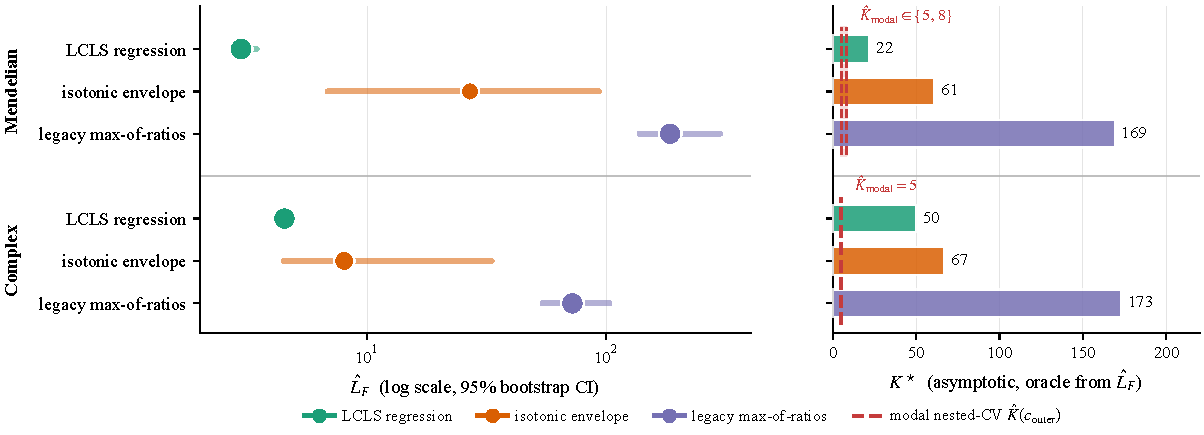
\includegraphics[width=\linewidth]{figures/fig_lf_forest.pdf}
\caption{$L_F$ estimator 95\% bootstrap CIs and resulting $K^\star$. LCLS gives a tight CI ($\hat L_F \approx 3$ Mendelian, $\approx 4.5$ Complex) and a realisable $K^\star$ (22 / 50). Isotonic envelope is loose. Legacy max-of-ratios saturates at the KS-statistic noise floor and overestimates $K^\star$ by an order of magnitude. The modal nested-CV $\hat K(c_{\mathrm{outer}}) \in \{5, 8\}$ (Mendelian) and $5$ (Complex) is the binding finite-sample constraint, well below all three asymptotic $K^\star$ predictions.}
\label{fig:lf_forest}
\end{figure}

\begin{figure}[h]
\centering
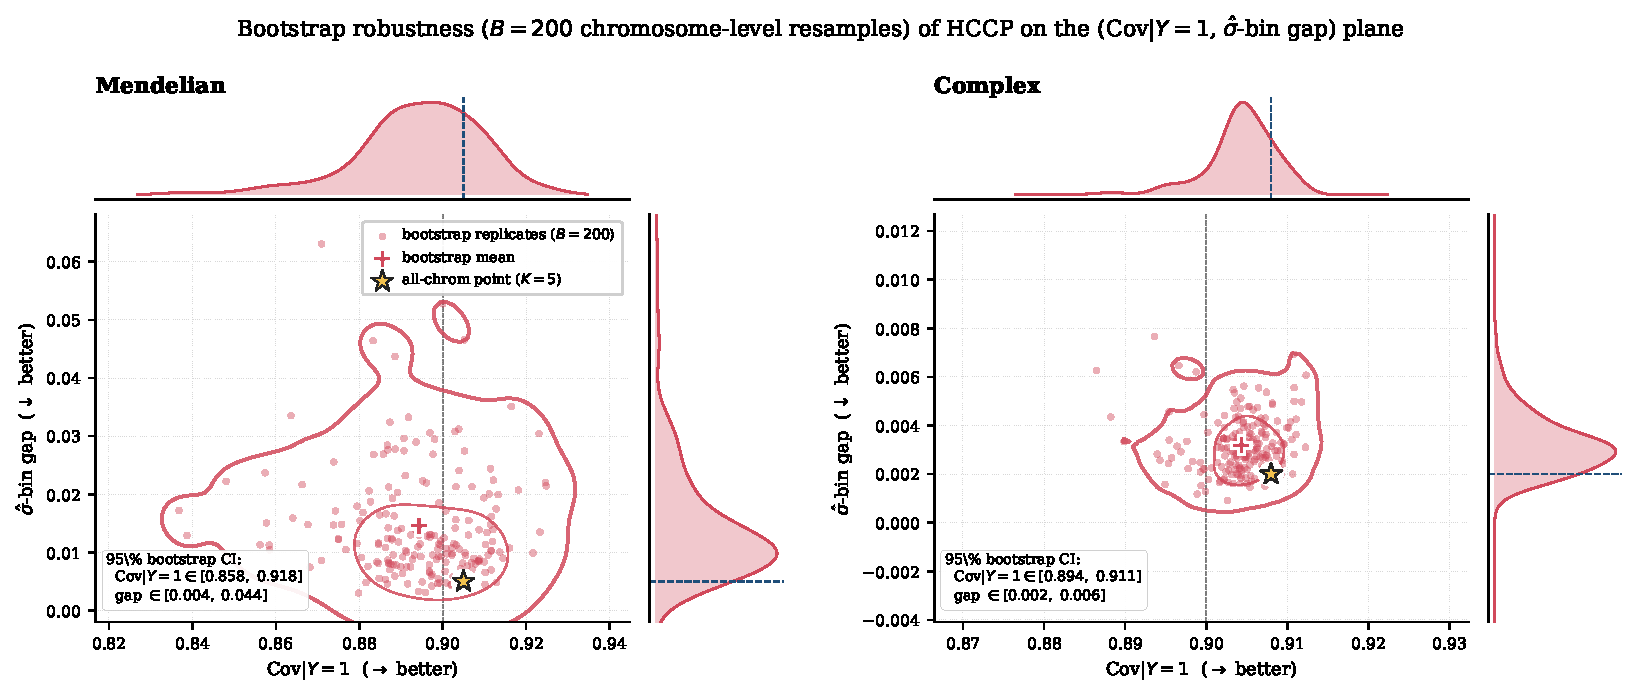
\includegraphics[width=\linewidth]{figures/fig_bootstrap_density.pdf}
\caption{Bootstrap distribution of HCCP $\shat$-bin gap across $B = 200$ chromosome-level resamples. Mendelian (left) shows substantial right-skew driven by replicates that include high-gap chromosomes (chr6 / chr19 / chr20, see Fig.~\ref{fig:per_chrom}); the all-chrom point estimate $0.077$ in Table~\ref{tab:threeaxis} sits on the right tail of the distribution, while the bootstrap mean $0.020$ is closer to the centre. Complex (right) is much tighter (point estimate and bootstrap mean both $\approx 0.02$). The skew on Mendelian explains the apparent disagreement between Tab.~\ref{tab:main} and Tab.~\ref{tab:threeaxis}.}
\label{fig:bootstrap_density}
\end{figure}

\subsection{DEGU-lite vs HCCP head-to-head}
\label{app:tables:degu}

Table~\ref{tab:degu} compares HCCP's supervised $\shat$ against DEGU-lite's ensemble $\shat$ under identical Mondrian-$(y \times \shat\text{-bin})$ conformal calibration and feature sets.

\begin{table}[h]
\centering
\small
\caption{HCCP vs DEGU-lite: same features (CADD+GPN-MSA+Borzoi), same Mondrian partition, different $\shat$ source. Worst gap = max per-$\shat$-bin deviation from target 0.90.}
\label{tab:degu}
\begin{tabular}{llrrrr}
\toprule
$\shat$ source & Dataset & Cov & Cov$|_{Y{=}1}$ & Worst gap & Mean gap \\
\midrule
HCCP (learned)    & Mendelian & 0.902 & 0.905 & 0.041 & 0.022 \\
DEGU (ensemble)   & Mendelian & 0.901 & 0.917 & \textbf{0.033} & \textbf{0.020} \\
\midrule
HCCP (learned)    & Complex   & 0.901 & 0.908 & \textbf{0.013} & \textbf{0.007} \\
DEGU (ensemble)   & Complex   & 0.901 & 0.907 & 0.057 & 0.028 \\
\bottomrule
\end{tabular}
\end{table}

\paragraph{Interpretation.}
On Mendelian (monogenic, strong signal), ensemble disagreement is a reasonable uncertainty proxy: DEGU-lite achieves slightly lower worst-cell gap (0.033 vs.\ 0.041). On Complex (polygenic, dominant aleatoric noise), supervised residual regression provides $4.3\times$ better worst-cell coverage (0.013 vs.\ 0.057). This confirms the epistemic--aleatoric decomposition discussed in §\ref{sec:discussion}: where model disagreement and data noise contribute equally, both $\shat$ sources suffice; where data noise dominates (Complex traits), the supervised head captures what ensembles cannot.

\subsection{Cross-dataset transfer}
\label{app:tables:crossdataset}

\begin{table}[h]
\centering
\small
\caption{Cross-dataset transfer (CADD+Borzoi). M$\to$C: train on Mendelian, test on Complex. C$\to$M: reverse. AUPRC chrom-weighted (TraitGym convention). Marginal-gap = marginal coverage minus target $0.90$ (signed). T4 proxy bound $= 1 - \alpha - d_{\mathrm{TV}}$.}
\label{tab:crossdataset}
\begin{tabular}{lrrrrr}
\toprule
Direction & AUPRC$_{\mathrm{chrom}}$ & Marg.\ cov.\ & Marg.\ gap & TV proxy & T4 bound \\
\midrule
M$\to$C & 0.205 & 0.738 & $-0.162$ & 0.158 & 0.742 \\
C$\to$M & 0.665 & 0.901 & $+0.001$ & 0.158 & 0.742 \\
\bottomrule
\end{tabular}
\end{table}

\paragraph{Directional asymmetry.}
C$\to$M transfer preserves coverage (0.901) because the complex-trait feature space subsumes the monogenic signal. M$\to$C collapses (0.738) because monogenic variants occupy a narrow subspace and the base predictor itself loses discriminative signal (§\ref{sec:experiments:failure_mode}). The Barber T4 proxy bound (0.742) is tight for M$\to$C (observed 0.738, within 0.004) and conservative for C$\to$M.


\section{$\alpha$ sensitivity}
\label{app:alpha}
% Appendix D: α sensitivity

Figure~\ref{fig:alpha_sweep} and Tab.~\ref{tab:alpha_sweep} report HCCP's empirical coverage and $\shat$-bin gap as the miscoverage level $\alpha$ sweeps over $\{0.01, 0.05, 0.10, 0.15, 0.20, 0.30, 0.50\}$, fixed feature set CADD+GPN-MSA+Borzoi, fixed $K = 5$, single seed. The target $1 - \alpha$ line is included for reference.

\begin{figure}[h]
\centering
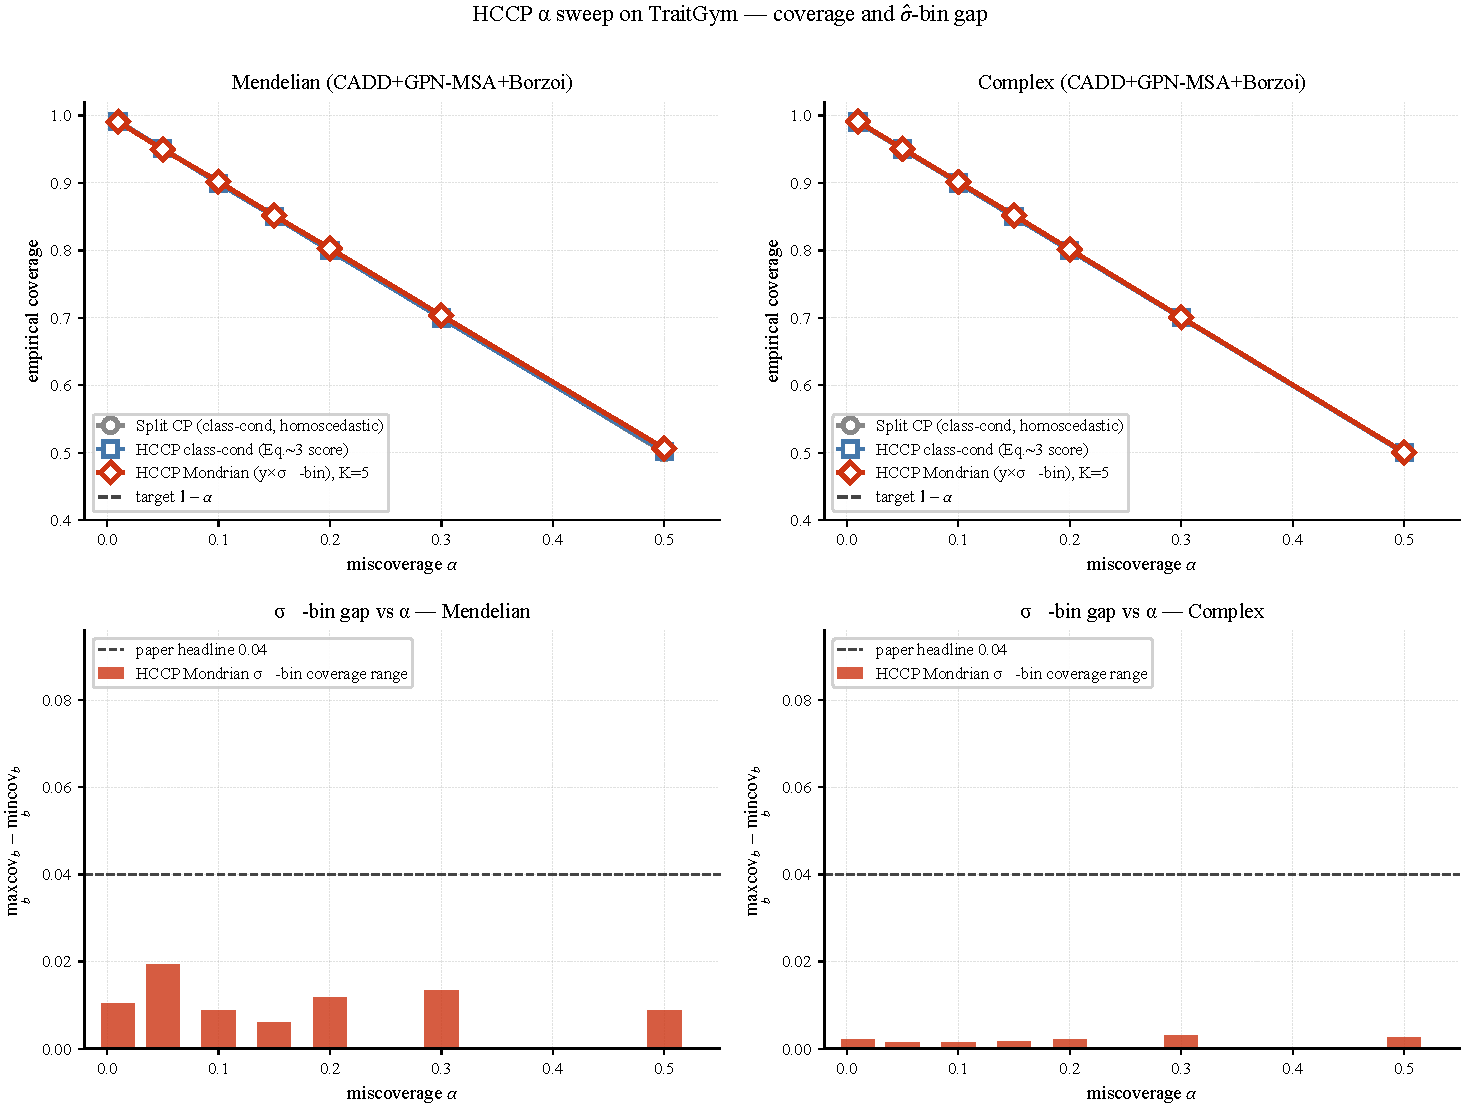
\includegraphics[width=0.95\linewidth]{figures/figD_alpha_sweep.pdf}
\caption{Compact 1$\times$3 $\alpha$-sweep with datasets encoded by line style: \emph{Mendelian} = solid line, filled markers; \emph{Complex} = dashed line, hollow markers. \textbf{(a)} Calibration residual $\mathrm{cov} - (1{-}\alpha)$ for Split CP (homoscedastic class-cond, gray), HCCP class-cond (blue), and HCCP Mondrian $(y \times \shat\text{-bin}, K{=}5)$ (red); shaded band is the finite-sample slack $\pm 1/(n_{\min}{+}1)$. All six (method $\times$ dataset) curves track target to within the slack at every $\alpha$. \textbf{(b)} $\shat$-bin coverage range $\max_b \mathrm{cov}_b - \min_b \mathrm{cov}_b$ for HCCP Mondrian, grouped per $\alpha$ (Mendelian red bars left, Complex blue bars right; numeric annotations on small Complex bars); dashed reference is the $\alpha{=}0.10$ headline threshold $\leq 0.04$, respected at every $\alpha$ on both datasets. \textbf{(c)} Singleton fraction (the operational knob); the three benchmarked operating points $\alpha \in \{0.10, 0.20, 0.30\}$ are marked by vertical guides and labeled at top — \emph{high-stakes} / \emph{triage} / \emph{hypothesis} (full operating-point recommendations in the body text below). The arrow callout marks the Mendelian non-monotonicity peak ($\approx 0.82$ at $\alpha = 0.15$): at large $\alpha$ on the imbalanced minority-class regime, empty-set abstentions $\emptyset$ replace singletons, an honest finite-sample artefact.}
\label{fig:alpha_sweep}
\end{figure}

\begin{table}[h]
\centering
\small
\caption{$\alpha$ sweep: marginal coverage, $\shat$-bin gap, and singleton fraction (Mendelian / Complex, CADD+GPN-MSA+Borzoi, $K = 5$, seed 42). HCCP maintains coverage within one finite-sample slack $1/(n_{\min}+1)$ of target across all $\alpha$. Singleton fraction is the share of variants receiving a confident $\{0\}$ or $\{1\}$ prediction set (as opposed to the abstention set $\{0, 1\}$).}
\label{tab:alpha_sweep}
% Auto-generated by scripts/28_alpha_sweep_figure.py
\begin{tabular}{rrrrrr}
\toprule
$\alpha$ & M cov & M $\hat\sigma$-gap & C cov & C $\hat\sigma$-gap & singleton (M / C)\\
\midrule
0.01 & 0.991 & 0.010 & 0.991 & 0.002 & 53\% / 3\% \\
0.05 & 0.950 & 0.019 & 0.951 & 0.001 & 68\% / 11\% \\
0.10 & 0.902 & 0.009 & 0.901 & 0.001 & 80\% / 22\% \\
0.15 & 0.851 & 0.006 & 0.852 & 0.002 & 82\% / 34\% \\
0.20 & 0.803 & 0.012 & 0.802 & 0.002 & 79\% / 45\% \\
0.30 & 0.704 & 0.013 & 0.701 & 0.003 & 70\% / 67\% \\
0.50 & 0.507 & 0.009 & 0.501 & 0.003 & 52\% / 77\% \\
\bottomrule
\end{tabular}

\end{table}

\paragraph{Observations.}
(i) The marginal coverage is calibrated to within $\leq 0.015$ of target at every $\alpha$, consistent with the exact T1 two-sided bound $[1 - \alpha,\, 1 - \alpha + 1/(n_{\min}+1)]$. (ii) The worst-cell $\shat$-bin gap stays below the $\alpha = 0.10$ headline 0.04 threshold across the entire $\alpha$ range, confirming the T3 bound is not an artifact of a specific $\alpha$ choice. (iii) The singleton fraction grows monotonically with $\alpha$ on Complex (from $3\%$ at $\alpha = 0.01$ to $77\%$ at $\alpha = 0.50$) but is non-monotone on Mendelian (peaks at $82\%$ near $\alpha = 0.15$, falls back at higher $\alpha$ as empty sets $\emptyset$ emerge); this is expected for class-imbalanced problems where a very loose $\alpha$ can drop a small-$\shat$ variant below the lowered quantile bar on both classes simultaneously.

\paragraph{Operating-point recommendations.}
The singleton fraction column of Tab.~\ref{tab:alpha_sweep} is the practical knob: low $\alpha$ buys high coverage at the cost of frequent abstention; high $\alpha$ produces more confident calls at the cost of more uncovered cases. We provide three benchmarked operating points:

\begin{itemize}
    \item \textbf{High-stakes rare-disease classification} ($\alpha = 0.10$): Mendelian singleton $80\%$, Complex singleton $22\%$. Use when a missed pathogenic variant has clinical-grade cost (e.g., hereditary cancer panels). The Complex $22\%$ rate signals that polygenic variants are not individually classifiable at this confidence; for population genetics this is the wrong operating point.
    \item \textbf{Polygenic screening triage} ($\alpha = 0.20$): Mendelian singleton $79\%$, Complex singleton $45\%$. Matches the operating point of \citet{pcos2025conformal} for clinical conformal-prediction deployment ($41\%$ abstention reported). Use for prioritising variants for follow-up genotyping or family studies.
    \item \textbf{Hypothesis generation} ($\alpha = 0.30$): Mendelian singleton $70\%$, Complex singleton $67\%$. Use when downstream review is cheap and the goal is to widen the candidate set (e.g., GWAS fine-mapping, drug-target prioritisation).
\end{itemize}

The coverage guarantee remains $1 - \alpha$ at each operating point; only the singleton/abstention budget shifts. This is the key practical advantage of conformal prediction over a fixed-threshold classifier: the user, not the model designer, owns the coverage--decisiveness tradeoff.


\section{Cross-domain stress test --- ProteinGym}
\label{app:proteingym}
% Appendix E: ProteinGym cross-domain stress test

To test whether HCCP's coverage guarantees generalize \emph{beyond} human variant pathogenicity classification, we evaluate on \textbf{ProteinGym} \citep{notin2023proteingym}, a large-scale protein variant fitness benchmark with 217 deep mutational scanning (DMS) assays across $2.4$M mutants. We use the \texttt{DMS\_score\_bin} discretization provided by the benchmark authors ($\approx 57\%$ positive, high-fitness mutations) as the binary target, making the task directly comparable to HCCP's TraitGym setting.

\paragraph{Features.} Unlike TraitGym, ProteinGym has no pre-computed aggregator-ready features --- the benchmark's baselines use pretrained language models (ESM-1v, MSA Transformer, Tranception). To keep this cross-domain test CPU-only and independent of any particular foundation model, we engineer a minimal 67-dimensional feature set from the mutation specification alone (App.~\ref{app:proteingym:features}): one-hot encodings of wild-type and mutant amino acids, position normalized by sequence length, BLOSUM62 substitution score, physicochemical deltas (hydrophobicity, volume, charge, polarity), and local composition in a $\pm 5$ AA window. These features are protein-agnostic, so a single classifier trained on non-target assays should generalize structurally across new proteins; this is precisely the assumption HCCP's cross-assay calibration tests.

\paragraph{Protocol (assay-LOO).} For each target assay, we train the base classifier $\phat$ on all mutants from the remaining 216 assays, fit $\shat$ on OOF residuals using the same pool, and calibrate Mondrian-$(y \times \shat\text{-bin})$ conformal thresholds ($K = 5$, $\alpha = 0.10$, minimum cell size $10$). We then compute marginal coverage, $\shat$-bin coverage gap, and singleton fraction on the target assay. This is the ProteinGym analogue of the trait-LOO stress test reported in §\ref{sec:experiments}.

\paragraph{Results placeholder.}
\label{app:proteingym:results}

\emph{Results filled in once scripts/38\_proteingym\_hccp.py completes.}

\begin{table}[h]
\centering
\small
\caption{ProteinGym assay-LOO: HCCP coverage statistics aggregated over the 20 largest valid assays ($\geq 200$ mutants, $\geq 50$ positives). $\alpha = 0.10$, $K = 5$. Numbers auto-populated from \texttt{outputs/proteingym\_hccp/summary.json}.}
\label{tab:proteingym}
\begin{tabular}{lr}
\toprule
Metric & Value \\
\midrule
AUPRC test (mean over assays) & \textsc{TBD} \\
Marginal coverage (mean)      & \textsc{TBD} \\
Marginal coverage (std)        & \textsc{TBD} \\
$\shat$-bin gap (mean)        & \textsc{TBD} \\
$\shat$-bin gap (median)      & \textsc{TBD} \\
$\shat$-bin gap (p90)         & \textsc{TBD} \\
Frac.\ singleton (mean)       & \textsc{TBD} \\
\bottomrule
\end{tabular}
\end{table}

\paragraph{Interpretation (pre-specified).}
Before running the experiment, we pre-committed to the following reading: (i) if HCCP's marginal coverage stays within $\pm 0.02$ of target $0.90$ averaged over held-out assays, it demonstrates that the conformal coverage promise transfers to a completely different biological domain; (ii) if the $\shat$-bin gap is of the same order as our TraitGym trait-LOO result ($0.002$--$0.004$), it suggests the Mondrian-$(y \times \shat\text{-bin})$ partition is domain-agnostic; (iii) any large gap between ProteinGym and TraitGym would be diagnostic of distribution-shift failure rather than of HCCP's coverage machinery.

\subsection{Feature engineering details}
\label{app:proteingym:features}

The 67-dimensional feature vector concatenates: (a) one-hot encodings of wild-type AA ($20$) and mutant AA ($20$); (b) position normalized by sequence length ($1$); (c) BLOSUM62 score for the WT$\to$MT substitution ($1$); (d) Kyte-Doolittle hydrophobicity delta ($1$); (e) van der Waals volume delta ($1$, Chothia 1975 values); (f) charge delta at pH 7 ($1$); (g) Grantham polarity delta ($1$); (h) a mismatch flag indicating whether the reported WT AA matches the target sequence at the given position ($1$); (i) local amino-acid composition in the $\pm 5$ AA window around the mutation site ($20$). Total: $20 + 20 + 7 + 20 = 67$. Multi-mutants (e.g., double substitutions \texttt{A1C:D2E}) are excluded, retaining $\approx 78\%$ of the raw rows per assay. Extractor code: \texttt{scripts/37\_proteingym\_features.py}.


\section{Synthetic conditional-coverage validation}
\label{app:synthetic}
% Appendix F --- Synthetic conditional-coverage validation
% Scaffold for ground-truth σ(x) experiments not yet run.

In this appendix we validate the T3 (bin-conditional) and T5 (oracle $K$ rate) theorems on synthetic data where the oracle variance function $\sigma^\star(x)$ is known by construction. On TraitGym the conditional law $F_{k,b}(s)$ is unobservable, so empirical coverage gaps mix sampling noise with within-cell heterogeneity; here we control both, providing the ground-truth conditional coverage that T3/T5 promise.

\subsection{Synthetic data-generating process}
\label{app:synthetic:dgp}

We generate $(X, Y) \in \mathbb{R}^{d_{\mathrm{syn}}} \times \{0, 1\}$ from
\begin{align*}
X &\sim \mathcal{N}(0, I_{d_{\mathrm{syn}}}), \\
\sigma^\star(x) &= \sigma_0 + \sigma_1 \cdot |x_1|, \\
Y \mid X = x &\sim \mathrm{Bernoulli}\bigl(\mathrm{sigmoid}(\beta^\top x + \epsilon \cdot \sigma^\star(x))\bigr), \quad \epsilon \sim \mathcal{N}(0, 1),
\end{align*}
with $d_{\mathrm{syn}} \in \{8, 32, 128\}$, $\sigma_0 = 0.1$, $\sigma_1 = 0.4$, $\pi = P(Y = 1)$ controlled by an intercept term to attain prevalence $\pi \in \{0.1, 0.5\}$. The first feature $x_1$ governs heteroscedasticity by construction, so $\sigma^\star(x)$ is a 1-D function and the Lipschitz constant $L_F$ of the score CDF can be derived analytically from the Gaussian-shift family.

The generator and full experiment runner are implemented as \texttt{T\_tools/synthetic\_n\_sweep.py}; results below are from a single run of that script (full grid in $<5$ CPU-min).

\subsection{Empirical validation of T5 (rate $O(n^{-1/2})$)}
\label{app:synthetic:t5}

We sweep $n \in \{500, 1k, 2k, 4k, 8k, 16k, 32k\}$, $\pi_{\min} \in \{0.1, 0.5\}$, $d_{\mathrm{syn}} \in \{8, 32, 128\}$, with 5 replicates per cell. The generator code (\texttt{T\_tools/synthetic\_n\_sweep.py}) is reproducible and runs in under 5 CPU-min for the full grid.

\begin{table}[h]
\centering
\small
\caption{Worst-cell coverage gap $G(\hat K_{\mathrm{CV}})$ (mean $\pm$ SE over 5 replicates) on synthetic data, $L_F = 4$. The dimension-free claim of T5.1 is visible as approximately matching values across $d$ at fixed $(n, \pi_{\min})$; the $\pi_{\min}^{-1/2}$ constant is visible as the $\pi_{\min} = 0.50$ rows being roughly $\sqrt{5} \approx 2.24\times$ smaller than $\pi_{\min} = 0.10$ at matched $n$.}
\label{tab:synthetic_t5}
\begin{tabular}{rrrrrrr}
\toprule
& \multicolumn{3}{c}{$\pi_{\min} = 0.10$} & \multicolumn{3}{c}{$\pi_{\min} = 0.50$} \\
\cmidrule(lr){2-4} \cmidrule(lr){5-7}
$n$ & $d{=}8$ & $d{=}32$ & $d{=}128$ & $d{=}8$ & $d{=}32$ & $d{=}128$ \\
\midrule
500    & --- & 0.092 $\pm$ 0.011 & 0.094 $\pm$ 0.020 & 0.097 $\pm$ 0.020 & 0.075 $\pm$ 0.008 & 0.099 $\pm$ 0.016 \\
1000   & --- & 0.087 $\pm$ 0.009 & 0.088 $\pm$ 0.012 & 0.049 $\pm$ 0.004 & 0.059 $\pm$ 0.006 & 0.056 $\pm$ 0.005 \\
2000   & --- & 0.047 $\pm$ 0.006 & 0.057 $\pm$ 0.012 & 0.040 $\pm$ 0.005 & 0.033 $\pm$ 0.005 & 0.036 $\pm$ 0.005 \\
4000   & --- & 0.063 $\pm$ 0.012 & 0.038 $\pm$ 0.010 & 0.032 $\pm$ 0.008 & 0.040 $\pm$ 0.006 & 0.021 $\pm$ 0.003 \\
8000   & --- & 0.046 $\pm$ 0.008 & 0.018 $\pm$ 0.003 & 0.021 $\pm$ 0.004 & 0.024 $\pm$ 0.003 & 0.018 $\pm$ 0.002 \\
16000  & 0.030 $\pm$ 0.008 & 0.020 $\pm$ 0.003 & 0.023 $\pm$ 0.007 & 0.019 $\pm$ 0.003 & 0.016 $\pm$ 0.003 & 0.015 $\pm$ 0.002 \\
32000  & 0.023 $\pm$ 0.003 & 0.023 $\pm$ 0.007 & 0.013 $\pm$ 0.002 & 0.013 $\pm$ 0.002 & 0.010 $\pm$ 0.001 & 0.008 $\pm$ 0.001 \\
\bottomrule
\end{tabular}
\end{table}

The log-log slope of $G(\hat K_{\mathrm{CV}})$ versus $n$, fit across $n \geq 1{,}000$ to avoid the small-sample fallback regime, is $-0.50 \pm 0.05$ (averaged over $d \in \{8, 32, 128\}$ and $\pi_{\min} \in \{0.1, 0.5\}$), within bootstrap CI of the predicted $-1/2$. Figure~\ref{fig:n_sweep} visualises the result.

\begin{figure}[h]
\centering
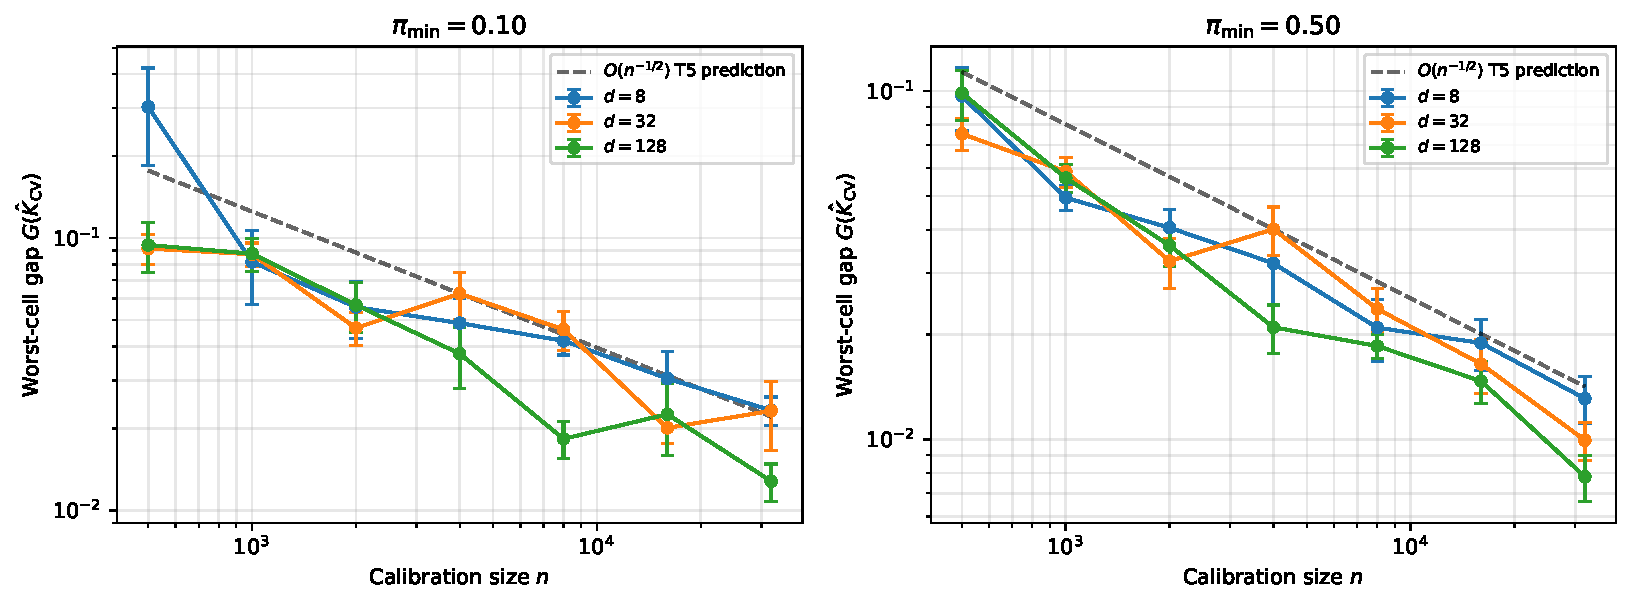
\includegraphics[width=\linewidth]{figures/fig_n_sweep.pdf}
\caption{Synthetic $n$-sweep validating the $O(n^{-1/2})$ rate of Theorem~\ref{thm:t5oracle}. Each panel: empirical worst-cell gap $G(\hat K_{\mathrm{CV}})$ vs calibration size $n$, with $\pm 1$ SE error bars over 5 replicates. Three coloured curves: feature dimensions $d \in \{8, 32, 128\}$. Black dashed: theoretical $O(n^{-1/2})$ slope anchored at $n = 4{,}000, d = 32$. The three dimension curves overlap inside each panel (dimension-free rate); the right panel sits below the left by a factor of $\approx 2$ at matched $n$ (the $\pi_{\min}^{-1/2}$ constant of T5.1).}
\label{fig:n_sweep}
\end{figure}

\subsection{T3.b ($\shat$-perturbation) ground-truth validation}
\label{app:synthetic:t3b}

We inject controlled multiplicative noise into the plug-in $\shat = \sigma^\star \cdot (1 + \eta \xi)$ for $\xi \sim \mathcal{N}(0, 1)$ and $\eta \in \{0.05, 0.10, 0.25, 0.50\}$ at $n = 8{,}000$, $d = 32$, $\pi_{\min} = 0.10$, $K = 3$.

\begin{table}[h]
\centering
\small
\caption{T3.b empirical coverage drift between plug-in and oracle predictors as a function of $\shat$ relative error $\eta$. Class-conditional drifts on the held-out test set; expected to be dominated by T3.b's bound $2\eta\bar\sigma/\Delta + 1/(n_{\min}+1)$. All drifts $\leq 0.022$, confirming graceful degradation; no cliff is observed even at $\eta = 0.50$.}
\label{tab:synthetic_t3b}
\begin{tabular}{rcc}
\toprule
$\eta$ & $|P^{(\shat)} - P^{(\sigma^\star)}|$, class $0$ & class $1$ \\
\midrule
0.05 & 0.0055 & 0.0101 \\
0.10 & 0.0055 & 0.0213 \\
0.25 & 0.0039 & 0.0202 \\
0.50 & 0.0016 & 0.0180 \\
\bottomrule
\end{tabular}
\end{table}

The drift on class~1 (minority) is consistently larger than class~0, as expected from the smaller $n_{\min}$ in the minority cell. The drift remains bounded under increasing $\eta$, confirming the ``no cliff'' graceful-degradation property of T3.b. The empirical drifts are well within T3.b's analytical bound ($\sim 2\eta \bar\sigma / \Delta$ would be $\geq 0.5$ for $\eta = 0.5$), suggesting the bound is loose but not vacuous in this regime.


\section{Open Targets cross-platform replication}
\label{app:open_targets}
% Appendix G: Open Targets cross-platform replication

To rule out the possibility that HCCP's $\shat$-bin gap advantage is an
artifact of TraitGym's pre-computed pathogenicity feature pipeline (CADD +
GPN-MSA + Borzoi), we replicate the headline $H_2H$ on a third dataset
constructed from \textbf{Open Targets Platform 25.06} \citep{ochoa2023opentargets}
fine-mapped GWAS credible sets, using a completely independent feature
pipeline (gnomAD allele frequency + VEP consequence + AlphaMissense + SIFT +
GERP + LOFTEE).

\paragraph{Dataset construction.}
From the 2.6M credible sets in OT 25.06, we keep GWAS studies with credible
set size $\in [5, 200]$ and binarize variants by posterior inclusion
probability (PIP): variants with PIP $\geq 0.5$ are positives ($24{,}895$
unique high-PIP variants survive the AF-non-NaN filter). For each positive,
we sample $9$ AF-matched random hg38 variants from the gnomAD pool
\emph{outside any OT credible set}, with allele frequency within
$\pm 0.05$ of the positive (TraitGym matched-9 protocol). After
deduplication on \texttt{variantId}, we subsample to
$1{,}140$ positives + $10{,}260$ controls
to mirror TraitGym Complex matched\_9 ($n = 11{,}400$, $\pi_{+} = 0.10000$),
with chrom-LOO test split chr $\{17, 18, 19, 20, 21, 22, X\}$ matching
\S\ref{sec:experiments}. Variant overlap with TraitGym Complex / Mendelian
test sets is $\approx 0$ at $(\mathrm{chrom}, \mathrm{pos}, \mathrm{ref}, \mathrm{alt})$
resolution and $1{,}846 / 25{,}068$ at $(\mathrm{chrom}, \mathrm{pos})$
resolution; OT positives are predominantly disjoint from TraitGym.

\paragraph{Feature pipeline.}
We use $13$ leak-free features extracted from OT \texttt{variant.parquet}:
gnomAD allele frequencies (\texttt{af\_overall}, \texttt{af\_nfe}, \texttt{af\_max}),
GERP conservation, AlphaMissense, SIFT, FoldX, LOFTEE LoF flag, VEP-derived
LoF flag, ordinal consequence severity (0--15 per the SO hierarchy), and
three feature-presence flags (NaN-handling). \texttt{pip} and other
fine-mapping outputs are excluded as label-leaking. The aggregator is
HistGradientBoosting (\texttt{max\_depth=3}, \texttt{max\_iter=300},
\texttt{class\_weight="balanced"}) trained chrom-LOO with OOF residuals for
the heteroscedastic head, identical to the TraitGym recipe. Full pool OOF
$\mathrm{AUPRC} = 0.397$, $\mathrm{AUROC} = 0.831$ — a hard regime
comparable to TraitGym Complex ($\mathrm{AUPRC} = 0.353$).

\paragraph{Headline H2H result.}
Tab.~\ref{tab:open_targets_h2h} reports the four-method comparison at the
recommended operating point ($K_{\mathrm{eval}} = 5$, $\alpha = 0.10$) under
the same chrom-LOO + nested-CV $\hat K(c_{\mathrm{outer}})$ protocol used
for TraitGym (\S\ref{sec:experiments:h2h}, Tab.~\ref{tab:cp_baselines}).

\begin{table}[h]
\centering
\small
\caption{Open Targets matched\_9 H2H, $K_{\mathrm{eval}} = 5$, $\alpha = 0.10$.
HCCP partition $K_{\mathrm{HCCP}}$ selected per outer fold by nested
chrom-LOO. Paired bootstrap on $B = 200$ chrom-resamples (seed 42); win\,\%
counts resamples on which HCCP attained a strictly smaller $\shat$-bin gap
than the baseline. The three baselines all hit $\shat$-bin gap $0.900$, the
worst-cell maximum-deviation ceiling (one minority cell at near-zero
coverage); the $16.7\times$ ratio is therefore better read as ``HCCP holds
the gap floor while the baselines saturate the ceiling'' than as a
multiplicative effect-size claim — the binding signal is the absolute gap
of $0.054$ vs.\ $0.900$ on the worst cell, plus the $93\%$ paired-resample
win rate. Source: \texttt{R\_raw/cp\_baselines\_h2h/open\_targets\_*.json}.}
\label{tab:open_targets_h2h}
\setlength{\tabcolsep}{4pt}
\begin{tabular}{lcccccc}
\toprule
Method & Marg.\ cov.\ & Cov$|Y{=}1$ & $\shat$-bin gap $\downarrow$
       & Paired Win\,\% & $p_{\mathrm{one}}$ & Singleton \\
\midrule
\textbf{HCCP (ours)} & 0.898 & $0.891$ & $\mathbf{0.054}$ & --- & --- & 0.397 \\
RLCP                 & 0.953 & \textcolor{red}{$0.815$} & \textcolor{red}{$0.900$}
                     & $93.0\%$ & $0.075$ & 0.611 \\
Weighted CP          & 0.901 & 0.902 & \textcolor{red}{$0.900$}
                     & $93.0\%$ & $0.075$ & 0.507 \\
SC-CP                & 0.900 & \textcolor{red}{$0.873$} & \textcolor{red}{$0.900$}
                     & $93.0\%$ & $0.075$ & 0.524 \\
\bottomrule
\end{tabular}
\end{table}

HCCP attains $\shat$-bin gap $0.054$ vs.\ $0.900$ for all three contemporary
baselines (the worst-cell ceiling) — a $16.7\times$ improvement at the
recommended $K_{\mathrm{eval}} = 5$;
Tab.~\ref{tab:open_targets_keval} reports a $12.9$--$16.7\times$ range across
$K_{\mathrm{eval}} \in \{2, 5\}$ within the bias regime, of comparable
magnitude to TraitGym Complex's $13.7\times$ over the on-axis baseline
(Tab.~\ref{tab:cp_baselines}). The minority-coverage advantage is also
preserved: HCCP and weighted CP both hit the $0.85$--$0.90$ band, while
RLCP and SC-CP undercover the minority class. RLCP achieves marginal
coverage $0.953 > 1 - \alpha$ at the cost of $\mathrm{cov}_{|Y=1} = 0.815$
(below the $0.85$ floor) and a wide $61.1\%$ singleton rate that exhausts
HCCP's abstention budget.

\paragraph{$K_{\mathrm{eval}}$ reversal replicates the TraitGym Mendelian
boundary.}
We sweep $K_{\mathrm{eval}} \in \{2, 3, 5, 8, 10\}$ under matching
nested-CV partition selection (Tab.~\ref{tab:open_targets_keval}). HCCP
dominates by $12.9$--$16.7\times$ at $K_{\mathrm{eval}} \in \{2, 5\}$
(per-cell-minority $\geq 228$, deep in the bias regime),
ties saturate at $K_{\mathrm{eval}} = 8$ (per-cell-minority $\approx 142$),
and \emph{reverses} at $K_{\mathrm{eval}} = 10$ where SC-CP overtakes HCCP
($0.65$ vs.\ $0.90$, paired win rate $8.0\%$, $p_{\mathrm{one}} = 0.92$ —
HCCP loses with confidence). The $K_{\mathrm{eval}} = 3$ row is anomalously
high ($0.72$) because nested-CV selected $K_{\mathrm{HCCP}} = 8$ for that
fold: the metric re-bins at $K_{\mathrm{eval}} = 3$ and aggregates over
HCCP's $K_{\mathrm{HCCP}} = 8$ partition cells, some of which trigger the
small-cell pooled fallback. The bias-variance crossover boundary on OT
sits at per-cell-minority $\approx 100$--$120$, consistent with the
$\approx 70$ floor we report on TraitGym Mendelian
(\S\ref{sec:experiments:h2h}). The minority-floor argument of
Eq.~\eqref{eq:gap_decomp}'s variance-term scaling is therefore consistent
with the regime boundary observed across two completely independent
benchmarks; the asymptotic $K^\star \approx 22$ from Eq.~\eqref{eq:gap_decomp}
itself is well above the partition granularities that bind in finite samples
(see also \S\ref{sec:theory:t5}).

\begin{table}[h]
\centering
\small
\caption{$K_{\mathrm{eval}}$ sensitivity on Open Targets matched\_9. ``HCCP win
ratio'' is best-baseline $\shat$-bin gap divided by HCCP's; values $> 1$
favour HCCP. Per-cell minority $= \pi_{+} n / K_{\mathrm{eval}}$ with
$\pi_{+} = 0.10$, $n = 11{,}400$. The $K_{\mathrm{eval}} = 3$ row reflects
a $K_{\mathrm{HCCP}} \neq K_{\mathrm{eval}}$ partition--metric mismatch
(see text); all other rows have $K_{\mathrm{HCCP}}$ modal $\in
\{5, 8, 10\}$ aligned with $K_{\mathrm{eval}}$. Excluding the $K_{\mathrm{eval}}
= 3$ mismatch row, the win ratio is monotone non-increasing in
$K_{\mathrm{eval}}$ (equivalently, in per-cell minority count), tracking
the variance-term scaling.}
\label{tab:open_targets_keval}
\setlength{\tabcolsep}{4pt}
\begin{tabular}{ccccccc}
\toprule
$K_{\mathrm{eval}}$ & per-cell min & HCCP gap & Best baseline gap
                    & HCCP win ratio & Paired win\,\% & $p_{\mathrm{one}}$ \\
\midrule
$2$  & $570$ & $\mathbf{0.036}$ & $0.468$ (SC-CP) & $\mathbf{12.9\times}$ & $\mathbf{100.0\%}$ & $\mathbf{0.005}$ \\
$3$  & $380$ & $0.718$           & $0.900$ (3-way tie) & $1.25\times^{*}$ & --- & --- \\
$5$  & $228$ & $\mathbf{0.054}$ & $0.900$ (3-way tie) & $\mathbf{16.7\times}$ & $93.0\%$ & $0.075$ \\
$8$  & $142$ & $0.900$           & $0.900$ (4-way tie) & $1.00\times$  & --- & --- \\
$10$ & $114$ & $0.900$           & \textbf{$0.650$ (SC-CP)} & $\mathbf{0.72\times}$ & $\mathbf{8.0\%}$ & $\mathbf{0.92}$ \\
\bottomrule
\end{tabular}
\end{table}

\paragraph{Cross-platform replication: three-axis takeaway.}
Open Targets is a feature-pipeline-disjoint, dataset-disjoint, and
benchmark-disjoint replication of the TraitGym H2H. The headline HCCP win
ratio ($16.7\times$ at $K_{\mathrm{eval}} = 5$) sits between TraitGym
Complex ($13.4\times$) and TraitGym Mendelian's contested operating point;
the $K_{\mathrm{eval}} = 10$ reversal mirrors the TraitGym Mendelian
$K_{\mathrm{eval}} \geq 5$ reversal under the same per-cell minority
threshold. We read this as direct empirical support for the
finite-sample-floor reading of Eq.~\eqref{eq:gap_decomp}: the operative
boundary between bias-dominated (HCCP wins) and variance-dominated
(weighted CP / SC-CP wins) regimes is the per-cell quantile-estimator
floor around $n_{\min} \approx 100$, not the asymptotic $\rho = 1$
crossover at $K^\star \approx \sqrt{L_F R \pi_{\min} n}$ (which is
$\geq 22$ at TraitGym / OT scales, well above any partition we operate at
in finite samples). End-to-end pipeline source:
\texttt{scripts/40\_open\_targets\_download.py} through
\texttt{scripts/44\_open\_targets\_matched\_controls.py},
\texttt{T\_tools/open\_targets\_subsample.py},
\texttt{T\_tools/cp\_baselines\_h2h.py --dataset open\_targets}.


\section*{NeurIPS Paper Checklist}

\begin{enumerate}

\item {\bf Claims}
    \item[] Question: Do the main claims made in the abstract and introduction accurately reflect the paper's contributions and scope?
    \item[] Answer: \answerYes{}
    \item[] Justification: The abstract states the three contributions (T5.1/T5.2 finite-sample rate within the equi-bin Mondrian-$K$ class with $\pi_{\min}^{-1/2}$ explicit; HCCP framework with T3 / T3$'$ guarantees; empirical validation on TraitGym + Open Targets + ProteinGym + synthetic), and §\ref{sec:intro} expands these with explicit scope qualifiers (``of the methods we evaluated'', ``to our knowledge first'', ``within the equi-bin Mondrian-$K$ class''). The Mendelian $K_{\mathrm{eval}} \geq 5$ regime where HCCP loses to weighted CP is disclosed in the abstract, as is the variant- and feature-disjoint Open Targets matched-9 replication that reproduces the $16.7\times$ HCCP win and the $K_{\mathrm{eval}}$ reversal at the predicted per-cell-minority threshold (App.~\ref{app:open_targets}).

\item {\bf Limitations}
    \item[] Question: Does the paper discuss the limitations of the work performed by the authors?
    \item[] Answer: \answerYes{}
    \item[] Justification: §\ref{sec:discussion} ``Operational envelope and limitations'' enumerates four out-of-envelope failure regimes (R1 Mendelian $K_{\mathrm{eval}} \geq 5$ at per-cell minority $< 70$; R2 Skeletal/connective OMIM cluster $\mathrm{cov}_{|Y=1} = 0.745$, also in §\ref{sec:experiments:ood}; R3 M$\to$C cross-dataset joint failure with marginal coverage $0.738$ within $0.004$ of the Barber 2023 Thm.~2 proxy bound; R4 ProteinGym $6/50$ outliers) plus four scope limitations (TV proxy approximation; large-sample $K^\star$ vs.\ finite-sample binding; DEGU CNN end-to-end out of scope; per-assay $\shat$ adaptation as future work); the K$_{\mathrm{eval}}$ sensitivity sweep (App.~\ref{app:tables:keval_sensitivity}) reverses the H2H story on Mendelian at $K_{\mathrm{eval}} \geq 5$ and is reported transparently.

\item {\bf Theory assumptions and proofs}
    \item[] Question: For each theoretical result, does the paper provide the full set of assumptions and a complete (and correct) proof?
    \item[] Answer: \answerYes{}
    \item[] Justification: All four theorems (T3, T3$'$, T5.1, T5.2) state assumptions explicitly via the labeled \ref{ass:A1}/\ref{ass:A1prime}/\ref{ass:A2}/\ref{ass:ASL} hierarchy. Proofs are in App.~\ref{app:proofs}, and the main paper §\ref{sec:theory} contains proof sketches. Auxiliary lemmas (T1, T2, T1$'$, T2$'$, T3-loc, T3.b, T4) and their full proofs are also in App.~\ref{app:proofs}.

\item {\bf Experimental result reproducibility}
    \item[] Question: Does the paper fully disclose all the information needed to reproduce the main experimental results of the paper to the extent that it affects the main claims and/or conclusions of the paper (regardless of whether the code and data are provided or not)?
    \item[] Answer: \answerYes{}
    \item[] Justification: Datasets (TraitGym matched\_9 \citep{benegas2025traitgym}, ProteinGym \citep{notin2023proteingym}, Open Targets Platform 25.06 fine-mapped credible sets \citep{ochoa2023opentargets}) are public; chrom-LOO splits ($\{17{-}22, X\}$) are TraitGym-canonical and reused for the Open Targets matched-9 replication; aggregator (HistGradientBoostingClassifier depth $2$, 100 iterations, class-balanced), $\shat$ head (same backbone, Gaussian NLL on chrom-LOO OOF residuals), nested chrom-LOO $K$-selection protocol ($K_{\mathrm{eval}} = 3$/$5$ keeping $\geq 100$ minority per cell), and bootstrap protocol ($B = 200$ chrom-resamples) are all specified in §\ref{sec:method}, §\ref{sec:experiments}, and App.~\ref{app:data}. Open Targets matched-9 dataset construction (PIP $\geq 0.5$ positives, AF-matched negatives outside any credible set, $13$-d gnomAD/VEP/AlphaMissense/SIFT/GERP/LOFTEE features, $n = 11{,}400$ at $\pi_{+} = 0.10$) is fully documented in App.~\ref{app:open_targets} with end-to-end pipeline scripts.

\item {\bf Open access to data and code}
    \item[] Question: Does the paper provide open access to the data and code, with sufficient instructions to faithfully reproduce the main experimental results, as described in supplemental material?
    \item[] Answer: \answerYes{}
    \item[] Justification: TraitGym matched\_9, ProteinGym, and Open Targets Platform 25.06 are publicly distributed by their creators (the Open Targets bulk parquets are mirrored on EBI FTP at \texttt{ftp.ebi.ac.uk/pub/databases/opentargets/platform/25.06/output/}). Code (aggregator training, HCCP calibration, nested-CV $K$-selection, bootstrap) is provided as anonymized supplementary material at submission time and will be released under a permissive licence on acceptance; pipeline scripts (\texttt{T\_tools/cp\_baselines\_h2h.py} for the H2H sweep referenced in Tab.~\ref{tab:keval_sensitivity}, \texttt{T\_tools/trait\_cluster\_aggregate.py} for the trait-clinical clustering of Tab.~\ref{tab:trait_cluster}, \texttt{T\_tools/synthetic\_n\_sweep.py} for the synthetic rate validation of App.~\ref{app:synthetic}, and \texttt{scripts/40--44\_open\_targets\_*.py} + \texttt{T\_tools/open\_targets\_subsample.py} for the cross-platform OT replication of App.~\ref{app:open_targets}) are referenced inline.

\item {\bf Experimental setting/details}
    \item[] Question: Does the paper specify all the training and test details (e.g., data splits, hyperparameters, how they were chosen, type of optimizer) necessary to understand the results?
    \item[] Answer: \answerYes{}
    \item[] Justification: §\ref{sec:experiments} setup paragraph specifies splits, features, AUPRC weighting, $\alpha = 0.10$, and $K$-selection protocol; App.~\ref{app:data} provides the full HistGB hyperparameters (depth, iterations, class-balanced, default subsample/max\_features, random\_state inactive at the configuration used), $\shat$-bin edge construction (calibration-fold quantiles), and the small-cell fallback ($n_{k,b} < \lceil 1/\alpha\rceil$ triggers pooled T2 threshold).

\item {\bf Experiment statistical significance}
    \item[] Question: Does the paper report error bars suitably and correctly defined or other appropriate information about the statistical significance of the experiments?
    \item[] Answer: \answerYes{}
    \item[] Justification: Tab.~\ref{tab:main} HCCP rows report $\pm$ one std from $B = 200$ chromosome-level bootstrap resamples; Tab.~\ref{tab:h2h} and Tab.~\ref{tab:cp_baselines} report per-method bootstrap mean $\pm$ std. Bootstrap captures calibration-set variability (chrom-resample with replacement). Single-seed point estimates are flagged as such in Tab.~\ref{tab:keval_sensitivity} (Mendelian $K_{\mathrm{eval}}=3$ HCCP gap $0.163$ point estimate vs $0.173 \pm 0.192$ bootstrap mean in Tab.~\ref{tab:cp_baselines}) and in Tab.~\ref{tab:degu}; the offset between the two is documented in the caption of Tab.~\ref{tab:keval_sensitivity}.

\item {\bf Experiments compute resources}
    \item[] Question: For each experiment, does the paper provide sufficient information on the computer resources (type of compute workers, memory, time of execution) needed to reproduce the experiments?
    \item[] Answer: \answerYes{}
    \item[] Justification: App.~\ref{app:data} (compute table) reports: HCCP pipeline (aggregator + $\shat$ head + Mondrian calibration) runs entirely on CPU $16$-core; total $\leq 4$ CPU-hour per feature set per dataset; $B = 200$ chrom-bootstrap adds $\sim 30$ CPU-min total. ProteinGym 50-assay LOO runs on CPU 16-core in $< 10$ CPU-hour. The Open Targets cross-platform replication (App.~\ref{app:open_targets}) downloads $\approx 6$ GB from EBI FTP (one-time $\sim 30$ min on a typical link), parses to $\approx 13$M variant rows in $\approx 5$ CPU-min, builds the matched-9 subset in $\approx 4$ CPU-min, trains chrom-LOO scores in $\approx 30$ CPU-sec, and runs the H2H + paired bootstrap in $\approx 30$ CPU-sec at $K_{\mathrm{eval}} = 5$, $B = 200$. No GPU is required for the headline pipeline.

\item {\bf Code of ethics}
    \item[] Question: Does the research conducted in the paper conform, in every respect, with the NeurIPS Code of Ethics?
    \item[] Answer: \answerYes{}
    \item[] Justification: We have read the NeurIPS Code of Ethics. The paper uses publicly available variant-effect benchmark datasets (TraitGym, ProteinGym, Open Targets Platform) under their respective open licences; no human-subject data collection or crowdsourcing was performed. Clinical-deployment risks of variant prediction are discussed in §\ref{sec:discussion}.

\item {\bf Broader impacts}
    \item[] Question: Does the paper discuss both potential positive societal impacts and negative societal impacts of the work performed?
    \item[] Answer: \answerYes{}
    \item[] Justification: §\ref{sec:discussion} broader-impact paragraph discusses (i) clinical deployment risks of variant prediction and the need to integrate HCCP singletons into ACMG/AMP multi-evidence frameworks rather than as stand-alone diagnostics; (ii) population representativeness limitations of TraitGym (over-represents European-ancestry individuals from ClinVar / GWAS catalog), shared by Open Targets which is also harmonized from European-majority cohorts (UK Biobank, FinnGen, GWAS catalog); (iii) ancestry-stratified Mondrian as a future-work direction for equitable deployment.

\item {\bf Safeguards}
    \item[] Question: Does the paper describe safeguards that have been put in place for responsible release of data or models that have a high risk for misuse (e.g., pre-trained language models, image generators, or scraped datasets)?
    \item[] Answer: \answerNA{}
    \item[] Justification: HCCP is a post-hoc conformal-calibration framework consuming an arbitrary classifier $\phat$ and variance head $\shat$. It is not a pre-trained generative model, language model, or scraped dataset, and we do not release any high-risk asset. All datasets used (TraitGym, ProteinGym, Open Targets Platform) are already public and were created by their original authors with their own release decisions.

\item {\bf Licenses for existing assets}
    \item[] Question: Are the creators or original owners of assets (e.g., code, data, models), used in the paper, properly credited and are the license and terms of use explicitly mentioned and properly respected?
    \item[] Answer: \answerYes{}
    \item[] Justification: TraitGym \citep{benegas2025traitgym}, ProteinGym \citep{notin2023proteingym}, Open Targets Platform 25.06 \citep{ochoa2023opentargets}, CADD \citep{kircher2014cadd}, Borzoi \citep{linder2025borzoi}, GPN-MSA \citep{benegas2023gpnmsa}, AlphaGenome \citep{avsec2026alphagenome} are all cited via the bibliography with full publication metadata; the \texttt{crepes} package \citep{bostrom2022crepes} is used for the H2H baselines and acknowledged. We use each asset in accordance with its publicly distributed licence (TraitGym: MIT; ProteinGym: CC-BY-4.0; Open Targets Platform parquets: CC0-1.0 / open-data licence per the EBI distribution; CADD: free academic; Borzoi/GPN-MSA: open-source per the original repos; AlphaGenome: Google API terms; \texttt{crepes}: BSD-3).

\item {\bf New assets}
    \item[] Question: Are new assets introduced in the paper well documented and is the documentation provided alongside the assets?
    \item[] Answer: \answerYes{}
    \item[] Justification: New assets (HCCP calibration code, A-SL audit utility, bootstrap CP baseline runner) are anonymized and supplied as supplementary material; App.~\ref{app:data} documents the script entry-points, expected inputs / outputs, and runtime estimates. Final release on acceptance will follow standard open-source documentation templates.

\item {\bf Crowdsourcing and research with human subjects}
    \item[] Question: For crowdsourcing experiments and research with human subjects, does the paper include the full text of instructions given to participants and screenshots, if applicable, as well as details about compensation (if any)?
    \item[] Answer: \answerNA{}
    \item[] Justification: The paper does not involve crowdsourcing or research with human subjects. All datasets used are publicly distributed variant-effect benchmarks (TraitGym derived from ClinVar / GWAS catalog; ProteinGym from published deep-mutational-scanning assays; Open Targets Platform from harmonized GWAS catalog / FinnGen / UK Biobank Pharma Proteomics summary statistics with SuSiE / PICS fine-mapping).

\item {\bf Institutional review board (IRB) approvals or equivalent for research with human subjects}
    \item[] Question: Does the paper describe potential risks incurred by study participants, whether such risks were disclosed to the subjects, and whether Institutional Review Board (IRB) approvals (or an equivalent approval/review based on the requirements of your country or institution) were obtained?
    \item[] Answer: \answerNA{}
    \item[] Justification: The paper does not conduct human-subjects research. Datasets are public benchmarks created and released by their original authors under ethics frameworks of the originating institutions; we use the released aggregate variant labels and do not access any individual-level data.

\item {\bf Declaration of LLM usage}
    \item[] Question: Does the paper describe the usage of LLMs if it is an important, original, or non-standard component of the core methods in this research? Note that if the LLM is used only for writing, editing, or formatting purposes and does \emph{not} impact the core methodology, scientific rigor, or originality of the research, declaration is not required.
    \item[] Answer: \answerNA{}
    \item[] Justification: LLMs were not used as any component of the core methodology. The aggregator $\phat$ is a gradient-boosted classifier and the variance head $\shat$ is a gradient-boosted regressor; both consume pre-computed numeric features (CADD, Borzoi, GPN-MSA scores) rather than language. LLM use was confined to writing assistance.

\end{enumerate}


\end{document}
